%\documentclass[compress]{beamer}
\documentclass[8pt]{beamer}

%-----------------------------------------------------------
% PACKAGES

%\usepackage[latin1]{inputenc}
\mode<presentation>

%\usepackage[T1]{fontenc}  
\usetheme{Warsaw}
%\usetheme{Madrid}

\usepackage{graphicx}
%\usepackage[section]{placeins} % force � mettre l'image o� on veut
%\usepackage{float} %utiliser H pour forcer � mettre l'image o� on veut
\usepackage{lscape} %utilisation du mode paysage
%\usepackage{pslatex}
\usepackage{url}
%\usepackage{subfigure}
\usepackage{caption}
\usepackage{subcaption}

\usepackage{graphicx}
\usepackage{tabls}
\usepackage{afterpage}

%\usepackage[]{media9}
\usepackage{multimedia}

\usepackage{amsthm}
\usepackage{amssymb}
\usepackage{amsmath}
\usepackage{amsfonts}
\usepackage{amstext}
\usepackage{amsbsy}
\usepackage{mathbbol} 


\usepackage{epsfig}
%\usepackage{epsfig}
%\usepackage{cites}
\usepackage{epsf}
\usepackage{array}
\usepackage{color}

%-----------------------------------------------------------
% NEW  DEFINITIONS
%
%=================================================================================================
% new commands
% +++++++++++++++++++++++++++++++++++++++++++++++++++++++++++++++++++++++++++++++++++++++++++++++++
\newcommand{\nc}{\newcommand}

\renewcommand{\div}{\mbold{\nabla}\! \cdot \!}
\newcommand{\grad}{\mbold{\nabla}}
\newcommand{\divv}[1]{\boldsymbol{\nabla}^{#1}\! \cdot \!}
\newcommand{\gradd}[1]{\mbold{\nabla}^{#1}}
\newcommand{\mbold}[1]{\boldsymbol#1}
% latex shortcuts
\newcommand{\bea}{\begin{eqnarray}}
\newcommand{\eea}{\end{eqnarray}}
\newcommand{\be}{\begin{equation}}
\newcommand{\ee}{\end{equation}}
\newcommand{\bal}{\begin{align}}
\newcommand{\eali}{\end{align}}
\newcommand{\bi}{\begin{itemize}}
\newcommand{\ei}{\end{itemize}}
\newcommand{\ben}{\begin{enumerate}}
\newcommand{\een}{\end{enumerate}}
\usepackage{amsthm}
\newtheorem*{remark}{Remark}
% DGFEM commands
\newcommand{\jmp}[1]{[\![#1]\!]}                     % jump
\newcommand{\mvl}[1]{\{\!\!\{#1\}\!\!\}}             % mean value
\newcommand{\keff}{\ensuremath{k_{\textit{eff}}}\xspace}
% shortcut for domain notation
\newcommand{\D}{\mathcal{D}}
% vector shortcuts
\newcommand{\vo}{\mbold{\Omega}}
\newcommand{\vr}{\mbold{r}}
\newcommand{\vn}{\mbold{n}}
\newcommand{\vnk}{\mbold{\mathbf{n}}}
\newcommand{\vj}{\mbold{J}}
\newcommand{\eig}[1]{\| #1 \|_2}
%
\newcommand{\EI}{\mathcal{E}_h^i}
\newcommand{\ED}{\mathcal{E}_h^{\partial \D^d}}
\newcommand{\EN}{\mathcal{E}_h^{\partial \D^n}}
\newcommand{\ER}{\mathcal{E}_h^{\partial \D^r}}
\newcommand{\reg}{\textit{reg}}
%
\newcommand{\norm}{\textrm{norm}}
\renewcommand{\Re}{\textrm{Re}}
\newcommand{\Pe}{\textrm{P\'e}}
\renewcommand{\Pr}{\textrm{Pr}}
%
\newcommand{\resi}{R}
%\newcommand{\resinew}{\tilde{D}_e}
\newcommand{\resinew}{\widetilde{\resi}}
\newcommand{\resisource}{\widetilde{\resi}^{source}}
\newcommand{\matder}[1]{\frac{\textrm{D} #1}{\textrm{D} t}}
%
\newcommand{\Gammakj}{\Gamma_{k \to j}}

% extra space
\newcommand{\qq}{\quad\quad}
% common reference commands
\newcommand{\eqt}[1]{Eq.~(\ref{#1})}                     % equation
\newcommand{\eqts}[1]{Eqs.~(\ref{#1})}                     % equations
\newcommand{\fig}[1]{Fig.~\ref{#1}}                      % figure
\newcommand{\tbl}[1]{Table~\ref{#1}}                     % table
\newcommand{\sct}[1]{Section~\ref{#1}}                   % section
\newcommand{\app}[1]{Appendix~\ref{#1}}                   % appendix
\newcommand{\lem}[1]{Lemma~\ref{#1}}                   % lemma
\newcommand{\theo}[1]{Theorem~\ref{#1}}                   % theorem
%
\newcommand{\ie}{i.e.,\@\xspace}
\newcommand{\eg}{e.g.,\@\xspace}
\newcommand{\psc}[1]{{\sc {#1}}}
\newcommand{\rs}{\psc{R7}\xspace}
%
\newcommand\br{\mathbf{r}}
%\newcommand{\tf}{\varphi}
\newcommand{\tf}{b}
%
%\renewcommand{\dim}{\ensuremath{\texttt{dim}}\xspace}
%
\newcommand{\tcr}[1]{\textcolor{red}{#1}}
\newcommand{\tcb}[1]{\textcolor{blue}{#1}}
  \newcommand{\tcg}[1]{\textcolor{green}{#1}}
\newcommand{\mt}[1]{\marginpar{ {\tiny #1}}}

\newtheorem{theorem}{Theorem}[section]
\newtheorem{lemma}[theorem]{Lemma}

\newcommand{\bs}[1]{\mathbf{#1}}
\renewcommand{\vec}[1]{\bs{#1}}
%\newcommand{\dd}{\mathrm{d}}
\newcommand{\norm}{\textrm{norm}}
\renewcommand{\Re}{\textrm{Re}}
\newcommand{\Pe}{\textrm{P\'e}}
\renewcommand{\Pr}{\textrm{Pr}}

\newcommand{\resi}{R_e}
%\newcommand{\resinew}{\tilde{D}_e}
\newcommand{\resinew}{\widetilde{\resi}}
\newcommand{\matder}[1]{\frac{\textrm{D} #1}{\textrm{D} t}}

\newcommand{\divv}[1]{\vec{\nabla}^{#1}\! \cdot \!}
\newcommand{\gradd}[1]{\vec{\nabla}^{#1}}

\newcommand{\tcr}[1]{\textcolor{red}{#1}}


%\newcommand{\resi}{R}
%\newcommand{\resinew}{\widetilde{\resi}}
\newcommand{\resisource}{\widetilde{\resi}^{source}}

\newcommand{\mbold}[1]{\boldsymbol#1}
%\newcommand{\norm}{\textrm{norm}}
\newcommand{\tcb}[1]{\textcolor{blue}{#1}}
\newcommand{\tcm}[1]{\textcolor{magenta}{#1}}
%\newcommand{\matder}[1]{\frac{\textrm{D} #1}{\textrm{D} t}}
\renewcommand{\thesubfigure}{\thefigure.\arabic{subfigure}}


%=================================================================================================

%============================================================

%style et couleur
%\usetheme{Frankfurt}
\date{\today}

%\addtobeamertemplate{footline}{\hfill\insertframenumber/\inserttotalframenumber\hspace{2em}\null}

\setbeamertemplate{footline}{
\leavevmode%
%\hbox{\hspace*{-0.06cm}
\begin{beamercolorbox}[wd=.5\paperwidth,ht=3.25ex,dp=1ex,center]{author in head/foot}%
	\usebeamerfont{author in head/foot}\insertshortauthor%~~(\insertshortinstitute)
\end{beamercolorbox}%
\begin{beamercolorbox}[wd=.25\paperwidth,ht=3.25ex,dp=1ex,center]{section in head/foot}%
	\usebeamerfont{section in head/foot} SIAM-CSE 2015 % \insertshorttitle
\end{beamercolorbox}%
\begin{beamercolorbox}[wd=.25\paperwidth,ht=3.25ex,dp=1ex,left]{section in head/foot}%
	\usebeamerfont{section in head/foot}\insertshortdate{}\hspace*{2em}
	\insertframenumber{} / \inserttotalframenumber %\hspace*{2ex}
\end{beamercolorbox}}%
%\vskip0pt%
%}

\beamertemplatetransparentcovered

\urldef{\ragusa}\url{jean.ragusa@tamu.edu}
\urldef{\delchini}\url{delcmo@tamu.edu}
\urldef{\berry}\url{ray.berry@inl.gov}

\title{An entropy-based viscous regularization for the seven-equation two-phase flow model}

\author{Jean C. Ragusa$^{\dagger,\ddagger}$, Marc O. Delchini$^\dagger$, Ray Berry$^\star$}
\institute{$^\dagger$Department of Nuclear Engineering, Texas A\&M University, College Station, TX\\
$^\ddagger$Institute for Scientific Computation, Texas A\&M University, College Station, TX\\
$^\star$Idaho National Laboratory, Idaho Falls, ID, TX}

%%%%%%%%%%%%%%%%%%%%%%%%%%%%%%%%%%%%%%%%%%%%%%%%%%%%%%%%%%%%%%%%%%%%

\begin{document}
%\renewcommand{\inserttotalframenumber}{\pageref{lastslide}}

\begin{frame}
\titlepage
\small{email: {\ragusa}, {\delchini}, {\berry}}

\end{frame}

\begin{frame}
	\frametitle{Outline}
	\tableofcontents 
\end{frame}

%%%%%%%%%%%%%%%%%%%%%%%%%%%%%%%%%%%%%%%%%%%%%%%%%%%%%%%%%%%%%%%%%%%%
%%%%%%%%%%%%%%%%%%%%%%%%%%%%%%%%%%%%%%%%%%%%%%%%%%%%%%%%%%%%%%%%%%%%
\section{Background and Motivation}
%%%%%%%%%%%%%%%%%%%%%%%%%%%%%%%%%%%%%%%%%%%%%%%%%%%%%%%%%%%%%%%%%%%%
%%%%%%%%%%%%%%%%%%%%%%%%%%%%%%%%%%%%%%%%%%%%%%%%%%%%%%%%%%%%%%%%%%%%

%%%%%%%%%%%%%%%%%%%%%%%%%%%%%%%%%%%%%%%%%%%%%%%%%%%%%%%%%%%%%%%%%%%%
\subsection{Next-generation nuclear reactor safety code}
%%%%%%%%%%%%%%%%%%%%%%%%%%%%%%%%%%%%%%%%%%%%%%%%%%%%%%%%%%%%%%%%%%%%

%%%%%%%%%%%%%%%%%%%%%%%%%%%%%%%%%%%%%%%%%%%%%%%%%%%%%%%%%%%%%%%%%%%%
\begin{frame}{RELAP (Reactor Excursion and Leak Analysis Program)}

\begin{block}{RELAP-5: Current industry and government standard in the US}
\begin{itemize}
\item 6-equation two-phase flow model with time- and volume-averaged equations. 
%The 6-eq model is ill-posed (non hyperbolic) and needs artificial viscosity and surface tension to be well-posed.
\item Semi-implicit in time with staggered spatial grids %(momentum grid half-shifted from the mass/energy grid)
\item Original model developed in the mid 1970s-early 1980s with continued enhancements since then.
\end{itemize}
\end{block}

\begin{block}{\tcm{RELAP-7}: next-generation reactor safety code}
\begin{itemize}
\item \tcr{Goal}: To leverage decades of advances in numerical methods and computer hardware
\item \tcr{Means}: Use the multiphysics framework \tcm{MOOSE} (Multiphysics Object-Oriented Simulation Environment) 
\begin{itemize}
\item Fully implicitly in time (BDF-2 time integration)
\item Jacobian-free Newton Krylov for nonlinear solves
\item Leverage from existing libraries: Finite Element Method (\tcm{libmesh}), linear/nonlinear solve libraries (\tcm{PETSc, Hypre}), meshing (Cubit), domain decomposition, ... 
\end{itemize}
\end{itemize}
\end{block}

\textbf{\underline{Our objective:} to develop an all-Mach numerical method for compressible single- and two-phase flow models that can be used with continuous schemes and implicit temporal integrators}


\end{frame}
%%%%%%%%%%%%%%%%%%%%%%%%%%%%%%%%%%%%%%%%%%%%%%%%%%%%%%%%%%%%%%%%%%%%

%%%%%%%%%%%%%%%%%%%%%%%%%%%%%%%%%%%%%%%%%%%%%%%%%%%%%%%%%%%%%%%%%%%%
\begin{frame}{MOOSE: Multiphysics Object-Oriented Simulation Environment}

\begin{block}{MOOSE}
\begin{itemize}
\item Open-source since March 2014: {\tt www.mooseframework.org}, 
\item R\&D Mag 100-award winners {\tt http://www.rdmag.com/award-winners/2014/07/2014-r-d-100-award-winners}
%\item \texttt{www.inl.gov/research/moose-applications/}
\end{itemize}

Many multiphysics \tcm{MOOSE-applications} already built using MOOSE:
\begin{enumerate}
\item BISON (thermo�mechanical fuel performance)
\item MARMOT (mesa-scale modeling of microscopic fuel changes during irradiation) 
\item RattleS$_\text{N}$ake ($S_N$ neutron transport)
\item RELAP-7 
\item \ldots
\end{enumerate}
\end{block}


\end{frame}
%%%%%%%%%%%%%%%%%%%%%%%%%%%%%%%%%%%%%%%%%%%%%%%%%%%%%%%%%%%%%%%%%%%%


%%%%%%%%%%%%%%%%%%%%%%%%%%%%%%%%%%%%%%%%%%%%%%%%%%%%%%%%%%%%%
\subsection{Density-based (compressible) Solvers for Low-Mach Flow Problems}
%%%%%%%%%%%%%%%%%%%%%%%%%%%%%%%%%%%%%%%%%%%%%%%%%%%%%%%%%%%%%%%%%%%%


%%%%%%%%%%%%%%%%%%%%%%%%%%%%%%%%%%%%%%%%%%%%%%%%%%%%%%%%%%%%%%%%%%%%
\begin{frame}{All-speed compressible fluid flow solver}

\vspace{-5mm}
\begin{block}{Viscous regularization }
\textcolor{magenta}{Artificial viscosity} schemes based on the entropy production 
 (Guermond et al., {\it Entropy viscosity method for nonlinear  conservation laws}, JCP-2011)\\
\smallskip
%The \tcm{entropy viscosity method} is \tcr{discretization-independent} and was significantly tested in the supersonic regime (including using \tcr{continuous FEM}).
The \tcm{Entropy Viscosity Method (EVM)} : \\
\hspace{0.5cm} $\bullet$ is \tcr{discretization-independent}  \\
\hspace{0.5cm} $\bullet$ was tested in the supersonic regime only \\
%\hspace{0.5cm} $\bullet$ was used on unstructured meshes  \\
%\hspace{0.5cm} $\bullet$ achieved \tcr{high-order accuracy} for smooth solution
%and was significantly tested in the supersonic regime
%(including using \tcr{continuous FEM}) . 
\end{block}
\vspace{-3mm}
\begin{block}{All-speed fluid flow solver}
\begin{itemize}
\item low-Mach flow $\rightarrow$ incompressible limit.
\item numerical methods developed for supersonic flows may fail to solve low-mach flows.
\begin{itemize}
\item derive a fix and keep dissipative terms well-behaved thru low-Mach asymptotic studies
\end{itemize}
\end{itemize}
Low-Mach: huge disparity in speeds (pressure waves move much faster)
\begin{itemize}
\item Severely CFL-constrained if using explicit time-stepping
\item Best to use \tcr{implicit} time stepping
\begin{itemize}
\item Nonlinear system of equations%(preconditioner: pressure-correction ICE, for example)\\
\item Fits the JFNK formalism in MOOSE % where all physic components are tightly coupled \\
\end{itemize}
\end{itemize}
\end{block}

\end{frame}
%%%%%%%%%%%%%%%%%%%%%%%%%%%%%%%%%%%%%%%%%%%%%%%%%%%%%%%%%%%%%%%%%%%%


%%%%%%%%%%%%%%%%%%%%%%%%%%%%%%%%%%%%%%%%%%%%%%%%%%%%%%%%%%%%%%%%%%%%
%%%%%%%%%%%%%%%%%%%%%%%%%%%%%%%%%%%%%%%%%%%%%%%%%%%%%%%%%%%%%%%%%%%%
\section{A Brief Review of the Entropy Viscosity Method for Conservation Laws}
%%%%%%%%%%%%%%%%%%%%%%%%%%%%%%%%%%%%%%%%%%%%%%%%%%%%%%%%%%%%%%%%%%%%
%%%%%%%%%%%%%%%%%%%%%%%%%%%%%%%%%%%%%%%%%%%%%%%%%%%%%%%%%%%%%%%%%%%%

%%%%%%%%%%%%%%%%%%%%%%%%%%%%%%%%%%%%%%%%%%%%%%%%%%%%%%%%%%%%%%%%%%%%
\subsection{Basic Idea}
%%%%%%%%%%%%%%%%%%%%%%%%%%%%%%%%%%%%%%%%%%%%%%%%%%%%%%%%%%%%%%%%%%%%


%%%%%%%%%%%%%%%%%%%%%%%%%%%%%%%%%%%%%%%%%%%%%%%%%%%%%%%%%%%%%%%%%%%%
\begin{frame}{Quick overview of the entropy-based artificial viscosity formalism}

General scalar conservation law: $\boxed{\partial_t u + \div \vec{f}(u) = 0}$.

\begin{enumerate}
\item Determine an entropy pair ($s(u),\, \vec{\Psi}(u)$) for the PDE under consideration
\item Compute the entropy residual $\boxed{R_e:=\partial_t s(u_h) + \div \Psi(u_h)}$, in each cell $K$, at each quadrature point $x_q$
\item Compute the speed associated with this residual
\be
v_e^K(x_q) := h_K \frac{|R_e(x_q)|_K}{|s-\overline{s}|_\infty}
\ee
%The denominator is used to normalize the residual
%. It is the deviation of $E(u)$ from the domain average $\overline{E}$.
\item Define the kinematic viscosity (m$^2$/s) as
\be
\mu^K(x_q) := h_K \min \Big( \frac{1}{2} \max_{x\in K}|\vec{f}'(u(x))|, \, v_e^K(x_q) \Big)
\ee
\item Plug in the standard Galerkin weak form as a \tcm{viscous regularization} %(\tcm{it is really a straightforward technique})
\be
\int_V \big( \partial_t u_h + \div \vec{f}(u_h) \big) b \, dx + \tcm{\sum_K \int_K \mu_K \grad u_h \cdot  \grad b \, dx} = 0 \quad \forall b
\ee
\end{enumerate}


\end{frame}
%%%%%%%%%%%%%%%%%%%%%%%%%%%%%%%%%%%%%%%%%%%%%%%%%%%%%%%%%%%%%%%%%%%%

%************************************************
\begin{frame}{Why an upper bound for viscosity?}

\begin{block}{}
Large entropy residual in shocks $\longrightarrow$ large entropy viscosity $\mu_e$ \\
\begin{center}
There is such a thing as too much of a good thing ...
\end{center}
\end{block}


\begin{block}{Upper bound for $\mu$}
First-order upwind scheme is monotone but over dissipative. We should not exceed the amount of stabilization that such a scheme provides.\\
\medskip
upwinding = \textcolor{blue}{centered approximation (Galerkin)} $-$ \textcolor{magenta}{numerical diffusion}\\
\underline{Example: linear advection} $\partial_t u + \beta \partial_x u =0$
\be
\beta \frac{u_i - u_{i-1}}{h} = \textcolor{blue}{\beta\frac{ u_{i+1}- u_{i-1}}{2h}} - \textcolor{red}{\frac{\beta h}{2}}
\textcolor{magenta}{\frac{ u_{i+1}-2u_i +u_{i-1}}{h^2}}
\ee
So, the dissipative term is $\frac{\beta h}{2}\partial_{xx} u$
and the first-order viscosity is $\frac{\beta h}{2}$
\end{block}

\begin{block}{First-order viscosity}
\hspace{0.5cm} $\bullet$ scalar conservation law: $\frac{h}{2}|f'(u)|$
\hspace{0.5cm} $\bullet$ system: $\frac{h}{2} \max \left( \text{eig}( \partial_u f) \right) $
\end{block}


\end{frame}
%%%%%%%%%%%%%%%%%%%%%%%%%%%%%%%%%%%%%%%%%%%%%%%%%%%%%%%%%%%%%%%%%%%%

%%%%%%%%%%%%%%%%%%%%%%%%%%%%%%%%%%%%%%%%%%%%%%%%%%%%%%%%%%%%%%%%%%%%
\subsection{Burger's equation}
%%%%%%%%%%%%%%%%%%%%%%%%%%%%%%%%%%%%%%%%%%%%%%%%%%%%%%%%%%%%%%%%%%%%

%************************************************
\begin{frame}{Example of application of the EVM: Burger's equation}

\begin{block}{The $1$-D Burger's equation with its viscous regularization}
\begin{equation}
\partial_t u(x,t) + \partial_x \left( \frac{u(x,t)^2}{2} \right) = \textcolor{blue}{\partial_x \left( \mu \left(x,t \right) \partial_x u(x,t) \right)} \nonumber
\end{equation}
\end{block}

\begin{block}{Definition of the local viscosity coefficient $\mu(x,t)$}
\begin{align}
&\mu(x,t) = \min \left( \mu_e(x,t), \mu_{max}(x,t) \right) \nonumber \\
&\mu_{max} (x,t) = \frac{h}{2} | u(x,t) | \nonumber \\
%&\mu_e(x,t) = h^2 \frac{\max \left( R(x,t), J \right)}{|| \eta(u) - \bar{\eta}(t) ||_\infty} \nonumber
&\mu_e(x,t) = h^2 \frac{ R(x,t)}{|| \eta(u) - \bar{\eta}(t) ||_\infty} \nonumber
\end{align}
\end{block}

\begin{block}{Entropy residual and jumps}
\hspace{0.5cm} $\bullet$ Entropy residual: $R(x,t) = \partial_t \eta(u) + \partial_x \Phi(u) \leq 0$ \\ 
\hspace{0.5cm} $\bullet$ with $ \eta(u) = u^2 / 2$  and $ \Phi(u) = u^3 / 3$ %\\
%\hspace{0.5cm} $\bullet$ Jumps:  $J = [[ \partial_n \Phi(u) ]] $
\end{block}
\end{frame}
%%%%%%%%%%%%%%%%%%%%%%%%%%%%%%%%%%%%%%%%%%%%%%%%%%%%%%%%%%%%%%%%%%%%


%************************************************
\begin{frame}{$1$-D numerical results (100 cells)} % and $t_f=0.24$ $s$)}
\begin{figure}[H]
        \centering
        \begin{subfigure}[b]{0.37\textwidth}
                \centering
                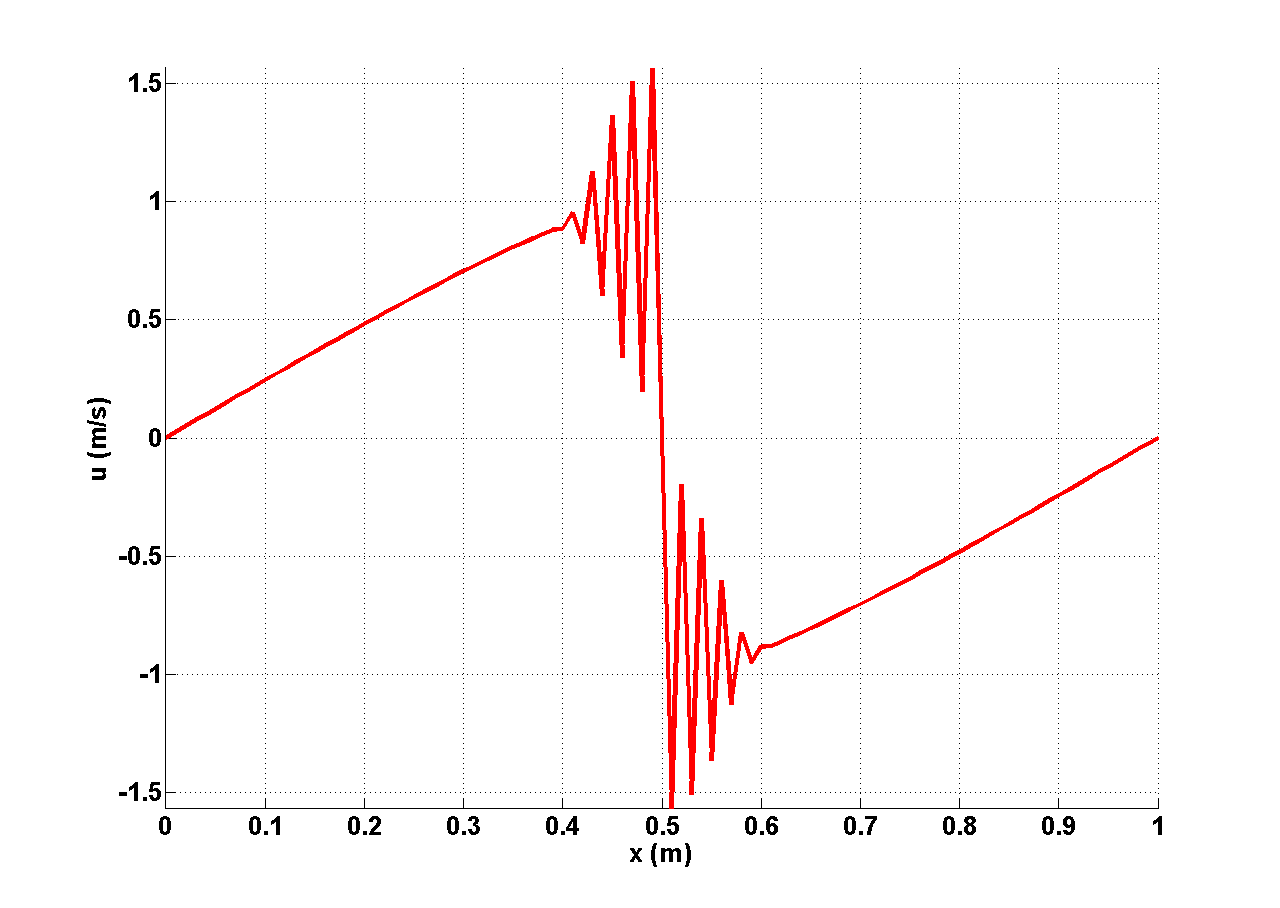
\includegraphics[width=\textwidth]{figures/1D_sol_free.png}
                \caption{Without stabilization.}
        \end{subfigure}% 
        %\begin{subfigure}[b]{0.37\textwidth}
                %\centering
                %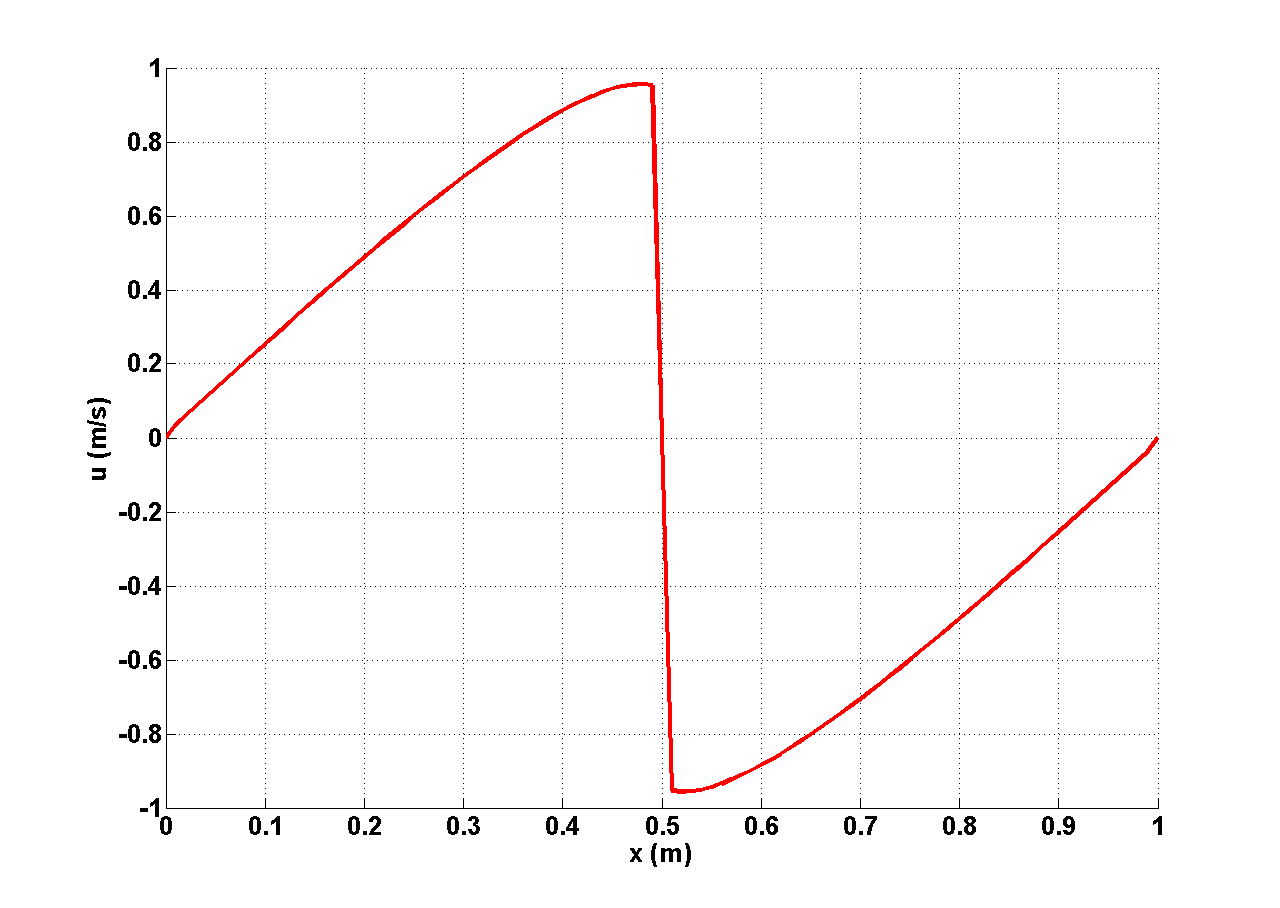
\includegraphics[width=\textwidth]{figures/1D_sol_fo.png}
                %\caption{With first-order viscosity.}
        %\end{subfigure}       
        \begin{subfigure}[b]{0.37\textwidth}
                \centering
                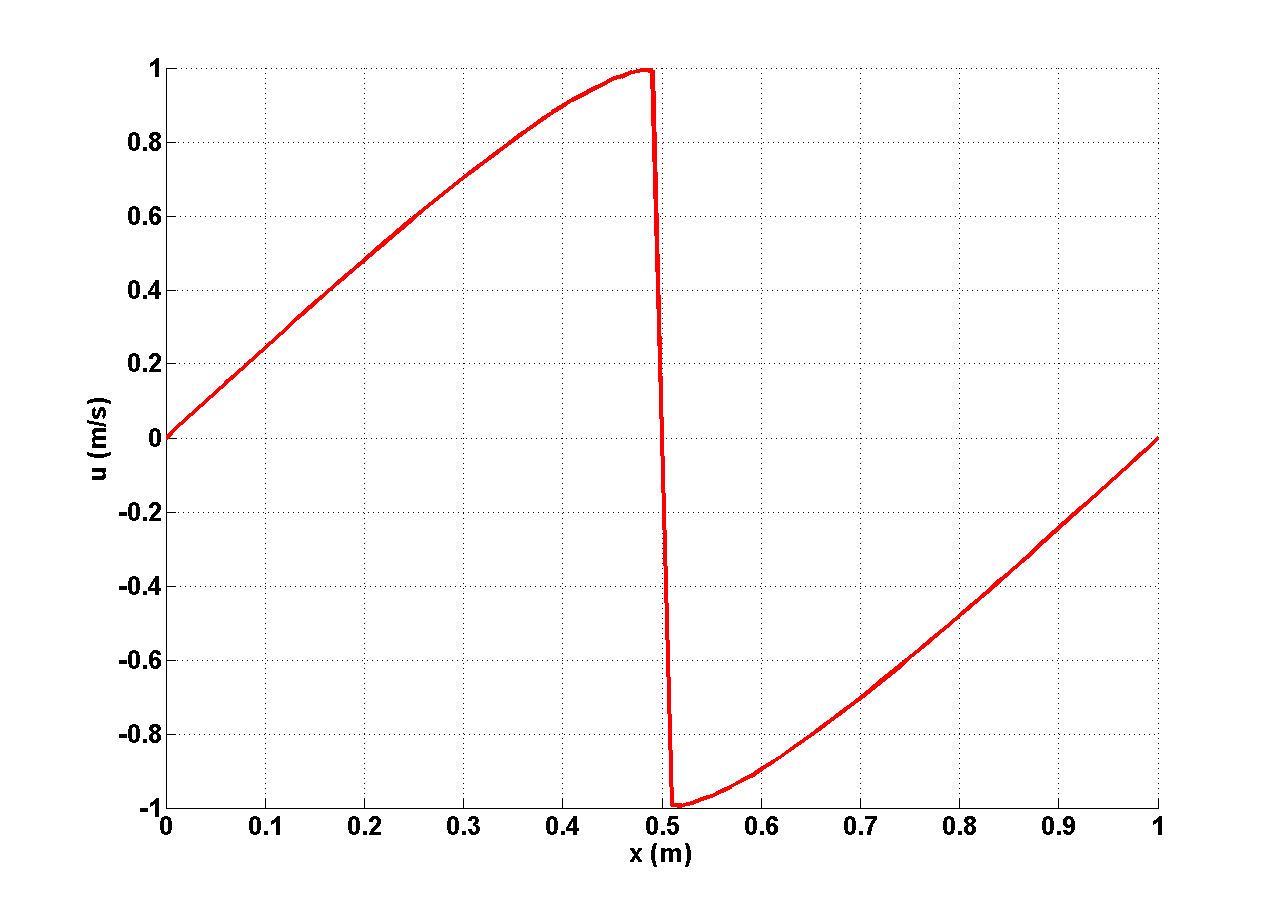
\includegraphics[width=\textwidth]{figures/1D_sol_ev.png}
                \caption{With the EVM.}
        \end{subfigure}
        \begin{subfigure}[b]{0.37\textwidth}
                \centering
                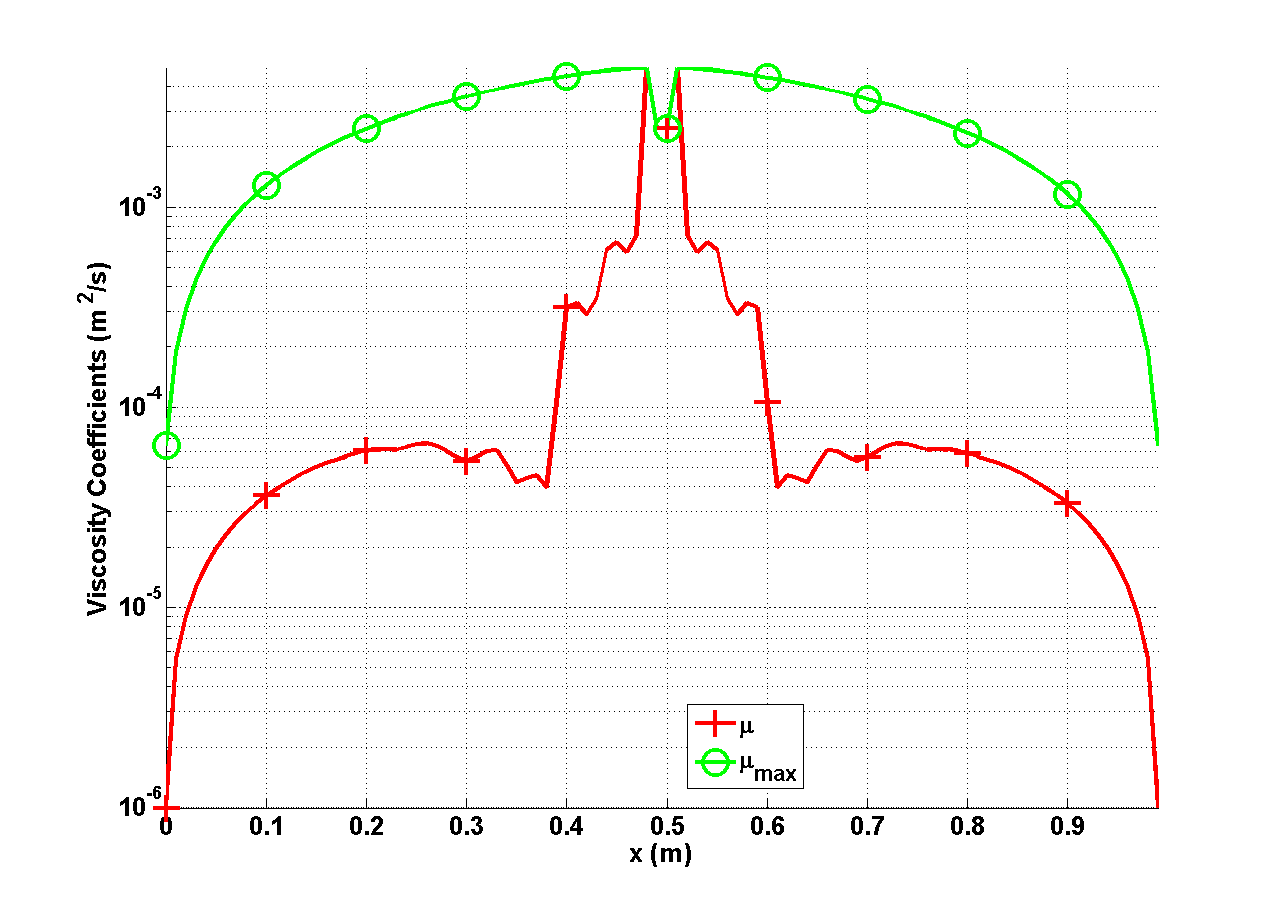
\includegraphics[width=\textwidth]{figures/1D_visc.png}
                \caption{Viscosity coefficient profiles.}
        \end{subfigure}
\end{figure}
\end{frame}

%************************************************
\begin{frame} 
%\frametitle{Example: Burgers equation}
%\begin{figure}
	%\includegraphics[height=7cm, keepaspectratio=true]{figs/burgers0000.png}
%\end{figure}
%\end{frame}
%
%\begin{frame} 
\begin{figure}
	\includegraphics[height=7cm, keepaspectratio=true]{figs/burgers20000.png}
\end{figure}
\end{frame}
%%%%%%%%%%%%%%%%%%%%%%%%%%%%%%%%%%%%%%%%%%%%%%%%%%%%%%%%%%%%%%%%%%%

%%%%%%%%%%%%%%%%%%%%%%%%%%%%%%%%%%%%%%%%%%%%%%%%%%%%%%%%%%%%%%%%%%%%
%%%%%%%%%%%%%%%%%%%%%%%%%%%%%%%%%%%%%%%%%%%%%%%%%%%%%%%%%%%%%%%%%%%%
\section{Single-phase Euler equations}
%%%%%%%%%%%%%%%%%%%%%%%%%%%%%%%%%%%%%%%%%%%%%%%%%%%%%%%%%%%%%%%%%%%%
%%%%%%%%%%%%%%%%%%%%%%%%%%%%%%%%%%%%%%%%%%%%%%%%%%%%%%%%%%%%%%%%%%%%

%%%%%%%%%%%%%%%%%%%%%%%%%%%%%%%%%%%%%%%%%%%%%%%%%%%%%%%%%%%%%%%%%%%%
%************************************************
\subsection{Entropy-viscosity method: original supersonic formulation}
%%************************************************

%%%************************************************
%\begin{frame}
%\begin{block}{\tcr{Regularized} Euler equations}
%\begin{subequations}
%\label{eq:euler_visc}
%%
%\begin{equation}
%\partial_t \rho + \div \left( \rho \vec{u} \right) = \textcolor{red}{\div \vec{f}} \nonumber
%\end{equation}
%%
%\begin{equation}
%\partial_t \left( \rho \vec{u} \right) + \div \left( \rho \vec{u} \otimes \vec{u} + P \mathbb{I} \right) =  \textcolor{red}{\div \mathbb{g} }\nonumber
%\end{equation}
%%
%\begin{equation}
%\partial_t \left( \rho E  \right) + \div \left[ \vec{u} \left( \rho E + P \right) \right] = \textcolor{red}{\div \vec{h} }\nonumber
%\end{equation}
%\end{subequations}
%
%\smallskip
%
%How to determine the \tcr{artificial viscous fluxes}?
%
%\smallskip
%
%By proving that the regularized equations satisfy a minimum principle on the specific entropy
%
%\end{block}
%
%\begin{block}{Minimum entropy principle}
%\be
%\inf_{x\in \mathbb{R}^d} s(x,t) \ge \inf_{x\in \mathbb{R}^d} s_0(x) \qquad \forall t \ge 0
%\ee
%\end{block}
%
%\end{frame}
%%%************************************************
%
%
%%%************************************************
%\begin{frame}{Idea of the derivation}
%
%\begin{block}{Entropy relationship: $\partial_t s + \vec{u} \cdot \grad s = \ldots $}
%Entropy is a function of internal energy $e$ and density $\rho$. Using chain rule, we have
%\[
%\partial_\alpha s = s_\rho \partial_\alpha \rho + s_e \partial_\alpha e \quad \text{ with } \alpha={t,x}
%\]
%Re-write Euler equations in non-conservative form as a function of $\rho$, $u$, and $e$
%\end{block}
%
%\begin{block}{Entropy equation}
%Use chain rule and the mass and internal energy equations to get:
%\begin{align}
%\rho \left( \partial_t s + \mbold{u} \cdot \grad s \right) = \div \left( \rho \kappa \grad s \right) -  \kappa \rho \mathbf{Q} +  s_e \mu \grad^s \mbold{u} : \grad \mbold{u} \nonumber
%\end{align}
%\end{block}
%%
%\begin{block}{Quadratic form}
%\begin{equation}
%\mathbf{Q} = X^t \mathbb{\Sigma} X 
%\quad \text{ with } 
%X = 
%\begin{bmatrix}
%\grad \rho \\
%\grad e 
%\end{bmatrix}
%\text{ and } 
%\mathbb{\Sigma} = 
%\begin{bmatrix}
       %\partial_{\rho} (\rho^2 \partial_{\rho} s) & \partial_{\rho,e} s  \\[0.3em]
       %\partial_{\rho,e} s & \partial_{e,e} s           \\[0.3em]
%\end{bmatrix} \nonumber 
%\end{equation}
%The form $Q$ is negative definite if and only if $-s$ is convex with respect to $e$ and $\rho^{-1}$.
%\end{block}
%\tcr{QED} \ \ (recall: $s_e = 1/T > 0 $)
%
%\end{frame}
%%%************************************************
%

%%************************************************
\begin{frame}
\begin{block}{Euler equations with viscous regularization (final form)}
\begin{subequations}
\label{eq:euler_visc}
%
%\text{Continuity equation:}
\begin{equation}
\partial_t \rho + \div \left( \rho \vec{u} \right) = \textcolor{red}{\div \left( \kappa  \grad \rho \right)} \nonumber
\end{equation}
%
%\text{Momentum equation:}
\begin{equation}
\partial_t \left( \rho \vec{u} \right) + \div \left( \rho \vec{u} \otimes \vec{u} + P \mathbb{I} \right) =  \textcolor{red}{\div \left( \mu \rho  \grad^s \vec{u}  + \kappa \vec{u} \otimes \grad \rho \right) }\nonumber
\end{equation}
%
%\text{Energy equation:}
\begin{equation}
\partial_t \left( \rho E  \right) + \div \left[ \vec{u} \left( \rho E + P \right) \right] = \textcolor{red}{\div \left( \kappa \grad \left( \rho e \right) + \frac{1}{2}|| \vec{u} ||^2 \kappa \grad \rho +  \rho \mu \vec{u} \grad \vec{u}  \right) }\nonumber
\end{equation}
\end{subequations}

\smallskip

where $\kappa$ and $\mu$ are positive viscosity coefficients.
\end{block}

Note that if $\mu = \kappa$ (and one selects $\grad \vec{u} $ instead of $\grad^s \vec{u} $), we recover a parabolic regularization (on $\rho$, $\rho \vec{u}$, and $\rho E$).

%\begin{block}{}
%\hspace{0.5cm} $\bullet$ Multi-wave problem: $\lambda_1 = \vec{u} \cdot \vec{n} - c $, $\lambda_2 = \vec{u} \cdot \vec{n} + c $ and $\lambda_{3, \dots, 3+D} = \vec{u} \cdot \vec{n}$. \\
%\hspace{0.5cm} $\bullet$ $\kappa$ and $\mu$ are two positive viscosity coefficients.
%\end{block}
\end{frame}
%%************************************************
%\begin{frame}
%\emph{Objectives: extend the EVM to low-Mach flows while maintaining its capabilities of solving for transonic and supersonic flows, and use an implicit solver.}
%\begin{block}{How to do it?}
%\begin{enumerate}
%\setlength{\itemsep}{10pt}
%\item recast the entropy equation as a function of the pressure, the density, the velocity and the speed of sound.
%\begin{equation}
%\mu_e(\vec{r},t) = h^2 \frac{\max \left( R(\vec{r},t), J \right)}{|| s - \bar{s}(t) ||_\infty} \nonumber
%\end{equation}
%%\item derive a viscous regularization for the multi-D Euler equations (Guermond and Popov (2014)) $\rightarrow$ extended to Euler equation with variable area.
%\item work with the non-dimensionalized version of the multi-D Euler equations in order to understand how the different terms scale
%%$\to$ will define non-dimensionalized numbers (Mach number, numerical Reynolds number, $\dots$)
%\item derive a definition for the viscosity coefficients that ensures well-scaled dissipative terms for a wide range of Mach numbers
%%$\to$ will consider two cases: isentropic and non-isentropic (with shocks) flows.
%\end{enumerate}
%\end{block}
%\end{frame}
%%************************************************
\begin{frame}{Supersonic formulation (Guermond, 2011)}
\vspace{-3mm}
\begin{block}{\textcolor{red}{Entropy-based viscosity coefficients} $\kappa_e$ and $\mu_e$ :}
\begin{itemize}
\item are based on the local entropy production,  
\item are numerically \tcm{evaluated} using the local entropy residual $\boxed{\resi(\vec{r},t) := \partial_t s + \vec{u} \cdot \grad s}$ %
%\begin{equation}
%\label{eq:ent_residual}
%\resi(\vec{r}, t) := \partial_t s + \vec{u} \cdot \grad s
%\end{equation}
\end{itemize}
%
\begin{equation}
\longrightarrow
\quad \mu^K_e(\vec{r}_q,t) =  h_K^2 \frac{  |\resi^K(\vec{r}_q,t) |}{|| s - \bar{s} ||_\infty}  
\qquad 
\kappa^K_e(\vec{r}_q,t) = \Pr \, \mu^K_e(\vec{r}_q,t)
\end{equation}
%
% $\Pr$ is a user-defined parameter and is usually taken in the range $[ 0.001; 1 ]$.
%\medskip

The denominator $|| s - \bar{s} ||_\infty$ is used for dimensionality purposes,
\textcolor{magenta}{no theoretical justification beyond a dimensionality argument}
\end{block}

\vspace{-1mm}
\begin{block}{First-order viscosities $\mu_{max}$ and $\kappa_{max}$}
\tcb{Upper bound} for the entropy viscosities  
%
\begin{equation}
\label{eq:fo}
\mu^K_{\max}(\vec{r}_q, t) = \kappa^K_{\max}(\vec{r}_q, t) = \frac{h}{2}  \left( || \vec{u}(\vec{r}_q, t) || + c(\vec{r}, t) \right)
\end{equation}
If $\mu^K_{\max}$ and $\kappa^K_{\max}$ are used, the discretization scheme is over-dissipative and first-order.
\end{block}
%
\vspace{-3mm}
\begin{block}{Viscosity definitions}
\be
\mu^K = \min (\mu^K_e , \mu^K_{\max}) \qquad \kappa^K = \min( \kappa^K_e , \kappa^K_{\max})
\ee
\end{block}

\end{frame}

%%************************************************
%%************************************************
\subsection{Low Mach approach}
%%************************************************
%%************************************************


%%************************************************
\begin{frame} 
\frametitle{\textcolor{red}{Low-Mach issues} with current viscosity definitions}

Recall that 

\begin{equation}
\mu^K_e(\vec{r}_q,t) =  h_K^2 \frac{|\resi^K(\vec{r}_q,t) |}{\textcolor{magenta}{|| s - \bar{s} ||_\infty}} 
%\qquad
%\kappa^K_e(\vec{r}_q,t) = \Pr \, \mu^K_e(\vec{r}_q,t)
\end{equation}


\begin{block}{Issues with current formulation in the low-Mach limit}
\begin{itemize}
\item In the low-Mach Regime, the flow is known to be \textcolor{red}{isentropic}, resulting in very little entropy production
\item In practice, the entropy residual $\resi$ will be very small in that regime  (i.e., small numerator in the expression for the viscosity coefficients)
\item and so will be the denominator $|| s - \bar{s} ||_\infty$,
\item Thus, the formula for the viscosity coefficients are not determined \textcolor{red}{(ill-scaled) in the low-Mach limit}
\end{itemize}
\end{block}

\end{frame}
%%********************************************************
\begin{frame}{Alternate definition of the entropy residual}

We can show that
\begin{equation}
\label{eq:ent_res}
\resi(\vec{r},t) := \partial_t s + \vec{u} \cdot \grad s = \matder{s} = \frac{s_e}{P_e} \underbrace{\left( \matder{P} - c^2 \matder{\rho} \right)}_{\resinew(\vec{r},t)} 
\end{equation} 

\underline{Idea for the demonstration:} 
$s$ is a function of $e$ and $\rho$, thus $\matder{s} = s_e\matder{e} + s_\rho \matder{\rho}$\\
\smallskip
Re-express the internal energy $e$ as a function of $P$ and $\rho$ through the EoS.

\begin{block}{Consequences}
\begin{itemize}
\item Residuals $\resi$ and $\resinew$ are proportional to one another\\
(for ideal gas law, $\frac{s_e}{P_e}= \frac{C_v}{P}$)
 %and will experience similar variations in space and time. 
\item We elect to employ $\resinew$ instead of $\resi$ %for the evaluation of the local entropy residual.
\item \tcr{{\it An analytical expression of the entropy function $s$ is no longer needed}} %: the residual $\resinew$ is evaluated using the local values of $P\,,\rho\,,u\,,c$ %pressure, density, velocity and speed of sound.
\item \textcolor{red}{Suitable normalizations for the residual} $\resinew$ can be devised (e.g., $P$, $\rho c^2$, $\rho c || \vec{u} ||$ or $\rho || \vec{u} ||^2$)%. Examples include the pressure itself or combinations of the density, the speed of sound and the norm of the velocity, i.e., $\rho c^2$, $\rho c || \vec{u} ||$ or $\rho || \vec{u} ||^2$. 
\end{itemize}
\end{block}
\end{frame}
%%********************************************************
\begin{frame}{What is a proper normalization for $\resinew(\vec{r},t)$?}

\begin{block}{Requirements} % {What is a proper normalization for $\resinew(\vec{r},t)$?}
\begin{enumerate}
\item To recover the incompressible results in the low-Mach limit (i.e., pressure fluctuations $\propto M^2$; divergence-free flow; incompressible continuity equation)
\item To remain valid and accurate for supersonic flows
\end{enumerate}

\end{block}

\smallskip 

We pose
\begin{equation}
\mu^K_e(\vec{r}_q,t)    = h_K^2 \frac{ | \resinew^K(\vec{r}_q,t) | }{\norm_P^\mu}    
%\end{equation} 
\quad
\text{and} 
\quad
%\begin{equation}
\kappa^K_e(\vec{r}_q,t) = h_K^2 \frac{ | \resinew^K(\vec{r}_q,t) | }{\norm_P^\kappa} 
\end{equation}

\bigskip

We now need to determine $\norm_P^\mu$ and $\norm_P^\kappa$. $\longrightarrow$
\textcolor{red}{Asymptotic analysis} to determine the proper scaling in the low-Mach limit.
%\textcolor{red}{Low-Mach Asymptotic analysis}. % to determine the viscosity coefficient scaling in the low-Mach limit.

\end{frame}
%%********************************************************
\begin{frame} 
\frametitle{Low-Mach Asymptotics: non-dimensionalization}

\begin{block}{Non-dimensionalized variables}

\begin{multline}
\label{eq:norm_param}
\rho^*   = \frac{\rho}{\rho_\infty}           ,\
u^*      = \frac{u}{u_\infty}                 ,\
P^*      = \frac{P}{\rho_\infty c^2_\infty}   ,\
E^*      = \frac{E}{c^2_\infty }              ,\\
x^* = \frac{x}{L_\infty}                      ,\
t^* = \frac{t}{L_\infty / u_\infty}           ,\ 
\mu^*    = \frac{\mu}{\mu_\infty}             ,\
\kappa^* = \frac{\kappa}{\kappa_\infty}       ,
\end{multline}
%
where  the subscript $\infty$ denote the far-field  quantities and the superscript $*$ stands for the non-dimensionalized variables.

\medskip

%The far-field reference quantities are chosen such that the dimensionless flow quantities are of order 1. 
%
%\medskip

The reference Mach number is given by
%
\begin{equation}
M_\infty = \frac{u_\infty}{c_\infty} ,
\end{equation}

\end{block}

\end{frame}
%%********************************************************
\begin{frame} 
\frametitle{Scaled Euler equations with viscous regularization}

\begin{subequations} 
\label{eq:Euler_eq2}
%
\begin{equation}
\label{eq:euler_eq2_cont}
\partial_{t^*} \rho^*+ \divv{*}  \left(  \rho^* \vec{u}^*  \right) = \frac{1}{\tcr{\Pe_\infty}} \divv{*}  ( \kappa^* \gradd{*} \rho^* )
\end{equation}
%
\begin{multline}
\label{eq:euler_eq2_mom}
\partial_{t^*} \left( \rho^* \vec{u}^* \right) 
+ \divv{*} \left( \rho^* \vec{u}^*\otimes \vec{u}^* \right) 
+ \frac{1}{\tcr{M_\infty^2}}\gradd{*}  P^*  
= 
\frac{1}{\tcr{\Re_\infty}} \divv{*} \left( \rho^* \mu^* \gradd{s,*} \vec{u}^* \right)  \\
+
\frac{1}{\tcr{\Pe_\infty}} \divv{*} \left(\vec{u}^*\otimes \kappa^* \gradd{*}  \rho^* \right)
\end{multline}
%
\begin{multline}
\label{eq:euler_eq2_energy}
\partial_{t^*} \left( \rho^* E^* \right) 
+ \divv{*}  \left[ \vec{u}^* \left( \rho^* E^* + P^* \right) \right] 
=
\frac{1}{\tcr{\Pe_\infty}} \divv{*}  \left( \kappa^*  \gradd{*} (\rho^* e^*) \right)   \\
+
\frac{\tcr{M_\infty^2}}{\tcr{\Re_\infty}} \divv{*}  \left( \vec{u}^* \rho^* \mu^* \gradd{s,*} \vec{u}^* \right)
+ 
\frac{\tcr{M_\infty^2}}{2 \tcr{\Pe_\infty}} \divv{*}  \left(\kappa^* (u^*)^2 \gradd{*} \rho^* \right) \, ,
\end{multline}
%
\end{subequations}

\medskip

\textcolor{magenta}{with the Reynolds $(\Re_\infty)$ and P\'eclet $(\Pe_\infty)$ numbers} :
%
\begin{equation}
\label{eq:ref_numb}
\boxed{\Re_\infty = \frac{u_\infty L_\infty}{\mu_\infty}} \quad \text{ and } \quad 
\boxed{\Pe_\infty = \frac{u_\infty L_\infty}{\kappa_\infty}} \, .
\end{equation}
%
%The Prandlt number used in the original version of the method is simply given by 
%\begin{equation} \label{eq:ref_nb_pr} 
%\Pr_\infty = \Pe_\infty / \Re_\infty \, .
%\end{equation}

\end{frame}
%%********************************************************
\begin{frame} 
\frametitle{\normalsize Low-Mach Asymptotics: How should $\Re$ and $\Pe$ scale with the Mach number?}

%\begin{block}{Expand each variable in powers of the Mach number}
%E.g.,
%%
%\begin{equation}
%\label{eq:expansion}
%P(\vec{r}, t) = P_0(\vec{r}, t) + P_1(\vec{r}, t) M_\infty + P_2(\vec{r}, t) M_\infty^2 + \dots 
%\end{equation}
%\end{block}

\begin{block}{Pressure spatial fluctuations}
To recover the low-Mach results that the leading order and first-order pressure terms ($P_0$ and $P_1$) are spatially constant, we require \textcolor{red}{$\Re_\infty = \Pe_\infty = 1$}. \\
$\longrightarrow$ pressure fluctuations $\propto M^2$
\end{block}

\begin{block}{Divergence of the flow}
With this scaling, one can also show that
\begin{equation}
\frac{1}{\gamma P_0} \frac{d P_0}{dt}=-\div \vec{u}_0
\quad \text{ and } \quad
\partial_t \rho_0 + \vec{u}_0 \cdot \div \rho_0 = 0 \, .
\end{equation}
$\longrightarrow$ steady-state divergence-free flows.
\end{block}

Therefore, by setting the $\Re_\infty=\Pe_\infty=1$, the \tcr{incompressible fluid results are retrieved in the low-Mach limit when employing the compressible Euler equations {\it with viscous regularization terms present}.}


\end{frame}
%%********************************************************
\begin{frame} 
\frametitle{Back to $\norm_P^\mu$ and $\norm_P^\kappa$}

From the definition of the entropy viscosity coefficient $\left( \kappa^K_e(\vec{r}_q,t)    = h_K^2 \frac{ | \resinew^K(\vec{r}_q,t) | }{\norm_P^\kappa} \right)$, we have
\begin{equation}
\label{eq:norm_relation}
\kappa_\infty 
= L_\infty^2  \frac{ \rho_\infty c_\infty^2 }{ L_\infty/u_\infty  \norm_{P,\infty}^{\kappa} }
\quad \to \quad \boxed{\norm_{P,\infty}^{\kappa} = \tcb{\Pe_\infty} \rho_\infty c_\infty^2} 
%= \frac{ \rho_\infty c_\infty^2 u_\infty L_\infty }{ \norm_{P,\infty}^{\kappa} } \, .
\end{equation}

Since $\tcb{\Pe}$ scales as \tcb{1},  we obtain:
%
\begin{equation}
\label{eq:norm_relation_bis}
\boxed{\norm_{P,\infty}^{\kappa} =  \rho_\infty c_\infty^2 } \, .
\end{equation}
%
\eqt{eq:norm_relation_bis} provides a proper normalization factor to define the $\kappa$ viscosity coefficient.\\

\medskip 
Similarly :  $\norm_{P,\infty}^{\mu} = \rho_\infty c_\infty^2 $.

\begin{block}{Thus, the new definitions for the viscosities in the low-Mach limit are}
\begin{equation}
\mu^K_e(\vec{r}_q,t)    = h_K^2 \frac{ | \resinew^K(\vec{r}_q,t) | }{ \rho_\infty c_\infty^2 }    \, ,
\quad
\text{and} 
\quad
\kappa^K_e(\vec{r}_q,t) = h_K^2 \frac{ | \resinew^K(\vec{r}_q,t) | }{ \rho_\infty c_\infty^2 } \, .
\end{equation}
\end{block}

\end{frame}
%%********************************************************
%%************************************************
%\begin{frame}{For a non-isentropic flow, i.e., with shocks}
%\begin{block}{Non-isentropic flows}
%\hspace{0.5cm} $\bullet$ the flow can experience shocks and other waves $\to$ discontinuities \\
%\hspace{0.5cm} $\bullet$ the low-Mach asymptotic study is no longer valid \\
%\hspace{0.5cm} $\bullet$ directly work with the non-dimensionalized Euler equations \\
%\hspace{0.5cm} $\bullet$ determine the scaling of $\Re_\infty$ and $\Pe_\infty$ to stabilize the equations \\
%%\item look at the low-Mach limit
%\end{block}{}
%%
%Non-dimensionalized momentum equation:
%\begin{align}
%\partial_{t} \left( \rho \vec{u} \right) 
%+ \div \left( \rho^* \vec{u}\otimes \vec{u} \right) 
%+ \textcolor{magenta}{\frac{1}{M_\infty^2}\grad  P}  
%= 
%\textcolor{blue}{\frac{1}{\Re_\infty} \div \left( \rho \mu \gradd{s} \vec{u} \right)} +
%\textcolor{blue}{\frac{1}{\Pe_\infty} \div \left(\vec{u}\otimes \kappa \grad  \rho \right)} \nonumber
%\end{align}
%\begin{block}{}
%In the shock region, the term $\textcolor{magenta}{\frac{1}{M_\infty^2}\grad  P}  $ will become dominant and will need to be stabilized by a dissipative term of the same scaling:
%\begin{itemize}
%\setlength{\itemsep}{10pt}
%\item (a) $\Re_\infty = M_\infty^2$ and $\Pe_\infty = 1$
%\item (b) $\Re_\infty = 1$ and $\Pe_\infty = M_\infty^2$
%\item (c) $\Re_\infty = \Pe_\infty = M_\infty^2$
%\end{itemize}
%$\longrightarrow$ each of the above options will affect the other equations (mass and energy equations).
%\end{block}
%\end{frame}
%%************************************************
%\begin{frame}{For a non-isentropic flow}
%Non-dimensionalized continuity equation:
%\begin{equation}
%\partial_{t} \rho+ \div  \left(  \rho \vec{u}  \right) = \textcolor{blue}{\frac{1}{\Pe_\infty} \div  ( \kappa \grad \rho )} \nonumber
%\end{equation}
%\begin{block}{choice (a) $\Pe_\infty = 1$}
%\begin{equation}
%\partial_{t} \rho+ \div  \left(  \rho \vec{u}  \right) = \textcolor{blue}{\div  ( \kappa \grad \rho )} \nonumber
%\end{equation}
%$\to$ the dissipative term is \emph{well-scaled}
%\end{block}
%\begin{block}{choice (b) and (c) $\Pe_\infty = M_\infty^2$}
%\begin{equation}
%\partial_{t} \rho+ \div  \left(  \rho \vec{u}  \right) = \textcolor{blue}{\frac{1}{M_\infty^2} \div  ( \kappa \grad \rho )} \nonumber
%\end{equation}
%$\to$ over-dissipation in the contact wave
%\end{block}
%Options (b) and (c) are not inappropriate. Thus, we are left with option (a): $\Re_\infty = M_\infty^2$ and $\Pe_\infty = 1$
%\end{frame}
%************************************************
\begin{frame}{Bridging the gap from low-Mach to supersonic}

\begin{block}{Answer from low-Mach asymptotic study}
\begin{equation}
\mu^K_e(\vec{r}_q,t)    = h_K^2 \frac{ | \resinew^K(\vec{r}_q,t) | }{ \rho c^2 }    \, ,
\text{ and }  
\kappa^K_e(\vec{r}_q,t) = h_K^2 \frac{ | \resinew^K(\vec{r}_q,t) | }{ \rho c^2 } \, .
\end{equation}
\end{block}

\begin{block}{Answer from non-isentropic study}
\begin{equation}
\mu^K_e(\vec{r}_q,t)    = h_K^2 \frac{ | \resinew^K(\vec{r}_q,t) | }{ \rho || \vec{u} ||^2 }    \, , \text{ and } 
\kappa^K_e(\vec{r}_q,t) = h_K^2 \frac{ | \resinew^K(\vec{r}_q,t) | }{ \rho c^2 } \, . \nonumber
\end{equation}
\end{block}

However, we want to keep the \textcolor{red}{all-speed aspect of the flow solver}, so

\begin{block}{New definitions}

\begin{subequations}
\begin{equation}
\mu^K_e(\vec{r},t)    = h_K^2 \frac{ | \resinew^K(\vec{r}_q,t) | }{\textcolor{magenta}{a(M) \rho \|\vec{u}\|^2 + (1-a(M)) \rho c^2}}  \, , \nonumber
\end{equation} 
\text{and} 
\begin{equation}
\kappa^K_e(\vec{r},t) = h_K^2 \frac{ | \resinew^K(\vec{r}_q,t) | }{ \rho c^2} \, . \nonumber
\end{equation}
\end{subequations}

\end{block}

\end{frame}

%%************************************************
\subsection{Numerical results}
%%************************************************

%%************************************************
\begin{frame}{Numerical results:}
%\begin{block}{$1$-D converging-diverging nozzle with Stiffened Gas EoS (backup slides)}
%$\longrightarrow$ steady-state exact solution $\to$ convergence study\\
%$\longrightarrow$ subsonic (liquid water) and supersonic (vapor) flows\\
%\end{block}

\begin{block}{$2$-D subsonic and transonic flows (with Ideal Gas EOS, $\gamma = 1.4$)}
$\longrightarrow$ low-Mach flow over a cylinder: $M_{inlet}=10^{-3}, 10^{-4}, 10^{-6} \text{ and } 10^{-7}$ \\
$\longrightarrow$ flow over a bump: $M_{inlet}=0.7, 10^{-2}, 10^{-4} \text{ and } 10^{-7}$
\end{block}

\begin{block}{$2$-D supersonic flow (with Ideal Gas EOS, $\gamma = 1.4$)}
Mach $3$ flow over a forward facing step
\end{block}

\end{frame}
%%************************************************
%\begin{frame}{$2$-D low-Mach flow over a cylinder}
%\begin{block}{Typical benchmark problem for low-Mach flow:}
%\begin{itemize}
%\item The steady-state solution is symmetric: the iso-Mach contour lines are used to asses the symmetry of the numerical solution
%\item The velocity at the top of the cylinder is twice the incoming velocity set at the inlet
%\item The pressure fluctuations are proportional to the square of inlet Mach number, i.e., 
%\begin{equation}
%\delta P = \frac{\max(P(\vec{r})) - \min(P(\vec{r}))}{\max(P(\vec{r}))}  \propto M_\infty^2 \nonumber
%\end{equation}
%where $\delta P$ and $M_\infty$ denote the pressure fluctuations and the inlet Mach number, respectively.
%\end{itemize}
%\end{block}
%\begin{block}{}
%\begin{itemize}
%\item triangular mesh with $4008$ triangular elements
%\item Ideal Gas equation of state with $\gamma = 1.4$
%\item CFL $= 20$
%\end{itemize}
%\end{block}
%\end{frame}
%************************************************
%\begin{frame}{$2$-D low-Mach flow over a cylinder}
%\begin{figure}[H]
%\centering
%\includegraphics[width=0.6\textwidth]{figures/Cylinder_geometry.png}
%\end{figure}
%\end{frame}
%************************************************
\begin{frame}{$2$-D low-Mach flow over a cylinder}
\begin{figure}
        \begin{subfigure}[b]{0.37\textwidth}
                \centering
                \includegraphics[width=\textwidth]{figures/CylinderMach1em3ZoomIn.png}
                \caption{$M_{\text{inlet}}=10^{-3}$}
        \end{subfigure}%
        \begin{subfigure}[b]{0.37\textwidth}
                \centering
                \includegraphics[width=\textwidth]{figures/CylinderMach1em4ZoomIn.png}
                \caption{$M_{\text{inlet}}=10^{-4}$}
        \end{subfigure}    
  
        \begin{subfigure}[b]{0.37\textwidth}
                \centering
                \includegraphics[width=\textwidth]{figures/CylinderMach1em6ZoomIn.png}
                \caption{$M_{\text{inlet}}=10^{-6}$}
        \end{subfigure}%
        \begin{subfigure}[b]{0.37\textwidth}
                \centering
                \includegraphics[width=\textwidth]{figures/CylinderMach1em7ZoomIn.png}
                \caption{$M_{\text{inlet}}=10^{-7}$}
        \end{subfigure}    
\end{figure}        
\end{frame}
%************************************************
\begin{frame}{$2$-D low-Mach flow over a cylinder}
\begin{figure}[H]
\centering
\includegraphics[width=0.9\textwidth]{figures/pressure_fluctuation.png}
\end{figure}
\end{frame}

%************************************************
\begin{frame}{$2$-D low-Mach flow over a bump}
\begin{figure}
        \begin{subfigure}[b]{0.5\textwidth}
                \centering
                \includegraphics[width=\textwidth]{figures/Hump2D_mach_0p7.png}
                \caption{$M_{\text{inlet}}=0.7$}
        \end{subfigure}%
        \begin{subfigure}[b]{0.5\textwidth}
                \centering
                \includegraphics[width=\textwidth]{figures/Hump2D_mach_0p01.png}
                \caption{$M_{\text{inlet}}=10^{-2}$}
        \end{subfigure}    
  
        \begin{subfigure}[b]{0.5\textwidth}
                \centering
                \includegraphics[width=\textwidth]{figures/Hump2D_mach_1em4.png}
                \caption{$M_{\text{inlet}}=10^{-4}$}
        \end{subfigure}%
        \begin{subfigure}[b]{0.5\textwidth}
                \centering
                \includegraphics[width=\textwidth]{figures/Hump2D_mach_1em7.png}
                \caption{$M_{\text{inlet}}=10^{-7}$}
        \end{subfigure}    
\end{figure}
\end{frame}
%%************************************************

%************************************************
%\begin{frame}{Fluid flow over a 2-D cylinder}
%\begin{table}[H]
%\begin{center}
 %\caption{\label{tbl:velocity_ratio}Velocity ratio for different Mach numbers.}
%\begin{tabular}{|c|c|c|c|}
%\hline
%Mach number & inlet velocity & velocity at the top of the cylinder & ratio \\ \hline
%$10^{-3}$ & $2.348$ $10^{-3}$ & $1.176$ $10^{-3}$& $1.99$  \\ \hline
%$10^{-4}$ & $2.285$ $10^{-4}$ & $1.145$ $10^{-4}$& $1.99$  \\ \hline
%$10^{-5}$ & $2.283$ $10^{-5}$ & $1.144$ $10^{-5}$ & $1.99$ \\ \hline
%$10^{-6}$ & $2.283$ $10^{-6}$ & $1.144$ $10^{-6}$ & $1.99$ \\ \hline
%$10^{-7}$ & $2.283$ $10^{-7}$ & $1.144$ $10^{-7}$ & $1.99$ \\ \hline
%\end{tabular}
%\end{center}
%\nonumber
%\end{table}
%\end{frame}
%************************************************
\begin{frame}{$2$-D Mach $3$ flow over a forward facing step}
  \begin{columns}
    \column{.5\textwidth}
    \movie[width=6cm,height=4cm,showcontrols=true,externalviewer]{\includegraphics[width=6cm,height=4cm]{engr.pdf}}{FFS_density_movie.mp4}\\
%       \includemedia[addresource=FFS_density_movie.mp4, activate=pageopen, deactivate=pageclose, width=6.5cm, height=5cm, flashvars={source=FFS_density_movie.mp4 & autoPlay=true & loop=true }]{}{VPlayer.swf}
    \column{.5\textwidth}
    \movie[width=6cm,height=4cm,showcontrols=true,externalviewer]{\includegraphics[width=6cm,height=4cm]{engr.pdf}}{FFS_viscosity_movie.mp4}\\
%      \includemedia[addresource=FFS_viscosity_movie.mp4, activate=pageopen, deactivate=pageclose, width=6.5cm, height=5cm, flashvars={source=FFS_viscosity_movie.mp4 & autoPlay=true & loop=true }]{}{VPlayer.swf}
  \end{columns}
%\begin{center}
%\movie[width=6cm,height=4cm,showcontrols=true,externalviewer]{\includegraphics[width=6cm,height=4cm]{engr.pdf}}{FFS_density_movie.mp4}\\
%\end{center}
\end{frame}
%\end{document}

%************************************************
%************************************************
\section{The seven-equation two-phase flow model}
%************************************************
%************************************************
%************************************************

\subsection{Description of the model}

%************************************************
\begin{frame}{The seven-equation model (SEM)}

\begin{block}{The model}
\begin{itemize}
\setlength{\itemsep}{10pt}
\item Each phase obeys the single-phase Euler equations: two continuity equations, two momentum equations and two energy equations
\item Seventh equation: volume fraction equation % $\rightarrow$ an internal boundary condition between the two phases at the interface
\item Exchange terms between phases: relaxation terms. These terms were derived using \emph{rational thermodynamic} and are consistent with the entropy minimum principle.
% $\rightarrow$ consistent with the entropy minimum principle
\item {\color{red}The system of equations is hyperbolic and has seven real waves}
\item The SEM degenerates to single-phase Euler equations when one phase disappears
\item The SEM degenerates into a 5-equation model when using infinite relaxation coefficients

\item \tcr{Numerical methods applied to the SEM : discontinuous schemes so far }
\end{itemize}
\end{block}

\end{frame}
%%************************************************
%\begin{frame}{The seven-equation model (SEM)}
%\begin{block}{Numerical stabilization methods}
%\begin{itemize}
%\setlength{\itemsep}{10pt}
%\item discontinuous schemes (finite volume, DG)
%\item approximate Riemann solvers: HLL, HLLC with low-Mach fix
%\item apply upwind-type scheme for non-conservative flux
%\end{itemize}
%\end{block}
%\begin{block}{Our approach}
%\begin{itemize}
%\setlength{\itemsep}{10pt}
%\item continuous scheme
%\item artificial dissipative method $\longrightarrow$ EVM
%\end{itemize}
%\end{block}
%\end{frame}
%%************************************************
%\begin{frame}{The seven-equation model (SEM)}
%\begin{block}{Methodology}
%\begin{enumerate}
%\item derive the entropy equation WITHOUT the dissipative terms
%\begin{align}
%(s_e)_k^{-1} \alpha_k \rho_k A \frac{d s_k}{dt} =& \textcolor{red}{\mu_P \frac{Z_k}{Z_k+Z_j} (P_j - P_k)^2} +
%\textcolor{red}{ \lambda_u \frac{Z_j}{Z_k+Z_j} (\mbold u_j - \mbold u_k)^2} \nonumber \\ 
%+& \textcolor{red}{|| \grad \alpha_k || \frac{Z_k }{\left( Z_k+Z_j \right)^2} \left[ Z_j (\vec{u}_j-\vec{u}_k)+\frac{\grad \alpha_k}{|| \grad \alpha_k ||}(P_k-P_j)\right]^2 }\nonumber
%\end{align}
%\item same steps as for the multi-D Euler equations: recast the entropy residual, viscous regularization, non-dimensionalized equations, viscosity coefficients.
%\end{enumerate}
%\end{block}
%\begin{block}{A particularity}
%Two phases $\to$ two entropy residuals $\to$ two options to derive the dissipative terms: \\
%(a) either we consider the total entropy residual by summing over the phases \\
%(b) or, we consider each phase independently of each other which will automatically ensure positivity of the total entropy \\
%\end{block}
%\end{frame}

\subsection{The entropy viscosity method applied to the Seven-Equation model}

%************************************************
\begin{frame}{Viscous regularization for the SEM (written here with variable area $A$)}

\begin{block}{}
\begin{subequations}
\begin{equation}
\partial_t \left( \alpha_k  A\right) + \vec{u}_{int} A \cdot \grad \alpha_k = {\color{red}A \mu_P \left( P_k - P_j \right)} + {\color{blue}\div \vec{l}_k}  
\end{equation}
%
\vspace{-2mm}
%
\begin{equation}
\partial_t \left( \alpha_k \rho_k A \right) + \div \left( \alpha_k \rho_k \vec{u}_k A \right) = {\color{blue}\div \vec{f}_k} 
\end{equation}
%
\vspace{-4mm}
%
\begin{multline}
\partial_t \left( \alpha_k \rho_k \vec{u}_k A \right) + \div \left[ \alpha_k A \left( \rho_k \vec{u}_k\otimes \vec{u}_k + P_k\mathbb{I}\right) \right] =   \\
\alpha_k P_k \grad A +  P_{int} A \grad \alpha_k +  {\color{red}A \lambda_u \left( \vec{u}_j - \vec{u}_k \right)} +{\color{blue}\div \mathbb{g}_k}
\end{multline}
%
\vspace{-4mm}
%
\begin{multline}
\partial_t \left( \alpha_k \rho_k E_k A \right) + \div \left[ \alpha_k A \vec{u}_j \left( \rho_k E_k + P_k \right) \right] =  \\
P_{int} \vec{u}_{int} A \grad \alpha_k - {\color{red}\mu_P \bar{P}_{int} \left( P_k-P_j \right)} +{\color{red}\bar{\vec{u}}_{int} A \lambda_u \left( \vec{u}_j - \vec{u}_k \right)} + {\color{blue}\div \vec{h}_k} 
\end{multline}
\end{subequations}
\end{block}
%
\vspace{-2mm}
%
\begin{block}{Viscous regularization: \tcm{same procedure} as with single-phase Euler equations}
\begin{equation}
\left\{
\begin{array}{lcl}
{\color{blue}\vec{l}_k} = A \beta_k \grad \alpha_k \\ %A {\color{magenta}\beta_k} \grad \alpha_k & & \\
{\color{blue}\vec{f}_k} = \alpha_k A {\color{magenta}\kappa_k}  \grad \rho_k + \rho_k \vec{l}_k& & \\
{\color{blue}\mathbb{g}_k} = \alpha_k A \rho_k {\color{magenta}\mu_k} \grad^s \vec{u}_k + \vec{u}_k \otimes \vec{f}_k & & \\
{\color{blue}\vec{h}_k} = \alpha_k A {\color{magenta}\kappa_k} \grad(\rho_k e_k) - \frac{||\vec{u}_k||^2}{2} \vec{f}_k + \vec{u} \cdot \mathbb{g}_k + \rho_k e_k \vec{l}_k & &
\end{array}
\right.
\nonumber
\end{equation}
Note: the viscous flux ${\color{blue}\vec{l}_k}$ plays no part in the entropy minimum principle; we used analogy with Burgers to determine it.
\end{block}
%Entropy equation:
%\begin{eqnarray}
%\alpha_k A \rho_k \frac{ds_k}{dt} + \left( {\color{green}\alpha_k A \kappa_k  \grad \rho_k} + {\color{red}\rho_k l_k} \right) \grad s_k - {\color{green}\div \left( \alpha_k A \rho_k \grad s_k \right)} = \nonumber \\ {\color{green}\partial_e s_k \alpha_k A \rho_k \mu_k \grad^s \vec{u} :  \grad \vec{u}}- {\color{green}X_k \Sigma_k X_k^t} + {\color{blue}Q}
%\nonumber
%\end{eqnarray}
\end{frame}
%************************************************
\begin{frame}{An all-Mach flow definition of the viscosity coefficients}
\begin{block}{\normalsize $\mu_k(\vec{r},t)    = \min \Big (\mu_{k,\max}(\vec{r},t), \mu_{k,e} (\vec{r},t)    \Big)$, and $\kappa_k(\vec{r},t) = \min \Big (\mu_{k,\max}(\vec{r},t), \kappa_{k,e} (\vec{r},t) \Big )$} 
\hspace{0.5cm} $\bullet$ $\ \kappa_{k,\max}(\vec{r},t)  = \mu_{k,\max} (\vec{r},t) = \frac{h}{2} \Big ( ||\vec{u}_k|| + c_k \Big )$.  \\ [3pt]
%
\hspace{0.5cm} $\bullet$ $\kappa_{k,e}(\vec{r},t) = \frac{h^2 \max(\resinew_k, J_k)}{ \textcolor{blue}{\rho_k c_k^2} }$ and
$\mu_{k,e}(\vec{r},t)    = \frac{h^2 \max(\resinew_k, J_k)}{ \textcolor{red}{\norm_{k,P}^\mu}}$  \\ [3pt]
%
\hspace{0.5cm} $\bullet$ $\resinew_k= \frac{DP_k}{Dt} - c_k^2 \frac{D\rho_k}{Dt}$ and $J_k = ||\vec{u_k} || \max \left( [[\ \grad P_k \cdot \vec{n}\ ]]  ,\ [[c_k^2 \grad \rho_k \cdot \vec{n} \ ]]\right)$ \\[3pt]
%
\hspace{0.5cm} $\bullet$ $\textcolor{red}{\norm_{k,P}^\mu} = \mathbb{G}(M_k) \rho_k || \vec{u}_k ||^2 + (1-\mathbb{G}(M_k)) \rho_k c_k^2$ \\ [4pt]
%
\hspace{0.5cm} $\bullet$ $\lim_{M_k \to 0} \mathbb{G}(M_k) = 0$ and $\lim_{M_k \to + \infty} \mathbb{G}(M_k) = 1$
%\hspace{0.5cm} $\bullet$ $\mathbb{G}(M_k) = \frac{\tanh (a(M_k-M_\infty)) + |\tanh (a(M_k-M_\infty))|}{2}$
\end{block}
%
\begin{block}{\normalsize $\beta_k(\vec{r},t) = \min \Big (\beta_{k,\max}(\vec{r},t), \beta_{k,e} (\vec{r},t) \Big )$}
\hspace{0.5cm} $\bullet$ $\beta_{max} = \frac{h}{2} || \vec{u}_{int} ||$ 
%and $\beta_{k,e} = h^2 \frac{\max( R_{k,\alpha}, J_{k,\alpha} )}{|| \eta_k - \bar{\eta}_k ||_\infty}$  \\ [3pt]
and $\beta_{k,e} = h^2 \frac{ R_{k,\alpha}}{|| \eta_k - \bar{\eta}_k ||_\infty}$  \\ [3pt]
\hspace{0.5cm} $\bullet$ $R_{k,\alpha} = \partial_t \eta_k + \vec{u}_{int}\cdot \grad \eta_k$ with $\eta_k = \frac{\alpha_k^2}{2}$ %and $J_{k,\alpha} = ||\vec{u}_{int} || \  [[\ \grad \alpha_k \cdot \vec{n}\ ]]$
\end{block}
\end{frame}
%************************************************
%\begin{frame}{How to derive the dissipative term $\vec{l}$ ?}
%\begin{equation}
%\partial_t \left( \alpha_k  A\right) + A \vec{u}_{int} \cdot \grad \alpha_k = {\color{blue}\div \vec{l}_k} \nonumber
%\end{equation}
%\begin{block}{}
%\begin{itemize}
%\item scalar hyperbolic equation with eigenvalue $\vec{u}_{int}$
%\item by analogy to the Burger's equation $\to$ $\vec{l}_k = A \beta_k \grad \alpha_k$
%\item this regularization ensures positivity of $\alpha_k$
%\item $\beta_k$ is a positive viscosity coefficient:
%\begin{align}
%&\beta_k = \min ( \beta_{k,e}, \beta_{max}) \text{ where }\nonumber \\
%&\beta_{max} = \frac{h}{2} || \vec{u}_{int} || \text{ and } \beta_{k,e} = h^2 \frac{\max( R_\alpha, J_\alpha )}{|| \eta - \bar{\eta} ||_\infty} \nonumber \\
%&R_\alpha = \partial_t \eta + \vec{u}_{int}\cdot \grad \eta \text{ with } \eta = \frac{\alpha_k^2}{2}  \nonumber
%\end{align}
%\end{itemize}
%\end{block}
%$\rightarrow$ when assuming $\mu_k = \kappa_k = \beta_k$, the parabolic regularization is retrieved
%\end{frame}
%%************************************************
%\begin{frame}{What about the viscosity coefficients $\mu_k$ and $\kappa_k$?}
%\begin{center}
%\textcolor{blue}{\Large{Same as single-phase equations}}
%\end{center}
%%\begin{subequations}
%%%
%%\begin{equation}
%%\mu_k(\vec{r},t)    = \min \Big (\mu_{\max ,k}(\vec{r},t), \mu_{e,k} (\vec{r},t)    \Big) \text{  and  }
%%\kappa_k(\vec{r},t) = \min \Big (\mu_{\max ,k}(\vec{r},t), \kappa_{e,k} (\vec{r},t) \Big ) \nonumber
%%\end{equation}
%%%
%%where the first-order viscosity is given by
%%\begin{equation}
%%  \kappa_{\max ,k}(\vec{r},t)  = \mu_{\max ,k} (\vec{r},t) = \frac{h}{2} \Big ( ||\vec{u}_k|| + c_k \Big ) \nonumber
%%\end{equation}
%%%
%%and the entropy viscosity coefficients by 
%%%
%%\begin{equation}
%%\kappa_{e,k}(\vec{r},t) = \frac{h^2 \max(\resinew_k, J_k)}{ \rho_k c_k^2 }  \text{  and  }
%%\mu_{e,k}(\vec{r},t)    = \frac{h^2 \max(\resinew_k, J_k)}{ \norm_{P,k}^\mu} \nonumber
%%\end{equation}
%%%
%%where
%%%
%%\begin{equation}
%%\norm_{P,k}^\mu =  \left\{
%%\begin{array}{ll}
%% \rho_k ||\vec{u}_k ||^2       & \text{ if } \left| \resinew_k^* \right| \geq M_k \text{ (i.e., non-isentropic flow)} \\
%% \rho_k c_k^2 = \norm_{P,k}^\kappa & \text{ otherwise} 
%%\end{array}
%%\right. \nonumber
%%\end{equation}
%%% 
%%with the jumps given by
%%%
%%\begin{equation}
%%J_k = || \vec{u}_k || \max \Big ( [[ \grad P_k \cdot \vec{n} ]], c_k^2 [[\grad \rho_k \cdot \vec{n}]] \Big) \nonumber
%%\end{equation}
%%\end{subequations}
%\end{frame}

\subsection{1-D numerical results}

%************************************************
\begin{frame}{Numerical results}
\begin{block}{}
\begin{itemize}
\setlength{\itemsep}{10pt}
\item $1$-D shock tube with two independent fluids
\item $1$-D shock tube with two fluids with pressure and velocity relaxation terms
\item 2-phase hydrostatic case
\item 2-phase water hammer
\end{itemize}
\end{block}
\end{frame}
%************************************************
\begin{frame}{$1$-D shock tube with two independent fluids}
\begin{block}{}
\begin{itemize}
\setlength{\itemsep}{5pt}
\item two fluids (1 and 2) described with ideal gas equation of state: $P = (\gamma-1) \rho e$
\item heavy fluid with $\gamma_1=3$ and light fluid with $\gamma_2 =1.4$
\item no interaction between the two fluids ($\mu_P=\lambda_u=0$) $\longrightarrow$ same as running a single-phase flow code twice
\item exact solution is available and obtained from a Riemann solver
\item $500$ cells, CFL$=1$ and $t_{flinal} = 305 \mu s$ 
\item initial step pressure: $P_{left} = 1 MPa$ and $P_{right} = 0.1 MPa$
\item fluids are initially at rest and uniform volume fraction $\alpha_i = 0.5$
\item uniform initial density $\rho_1 = 10 kg \cdot m^{-3}$ and $\rho_2 = 1 kg \cdot m^{-3}$
\end{itemize}
\end{block}
Objective: verify that the dissipative terms does not affect the volume fraction profile
\end{frame}
%************************************************
\begin{frame}{$1$-D shock tube with two independent fluids}
\begin{figure}
        \begin{subfigure}[b]{0.37\textwidth}
                \centering
                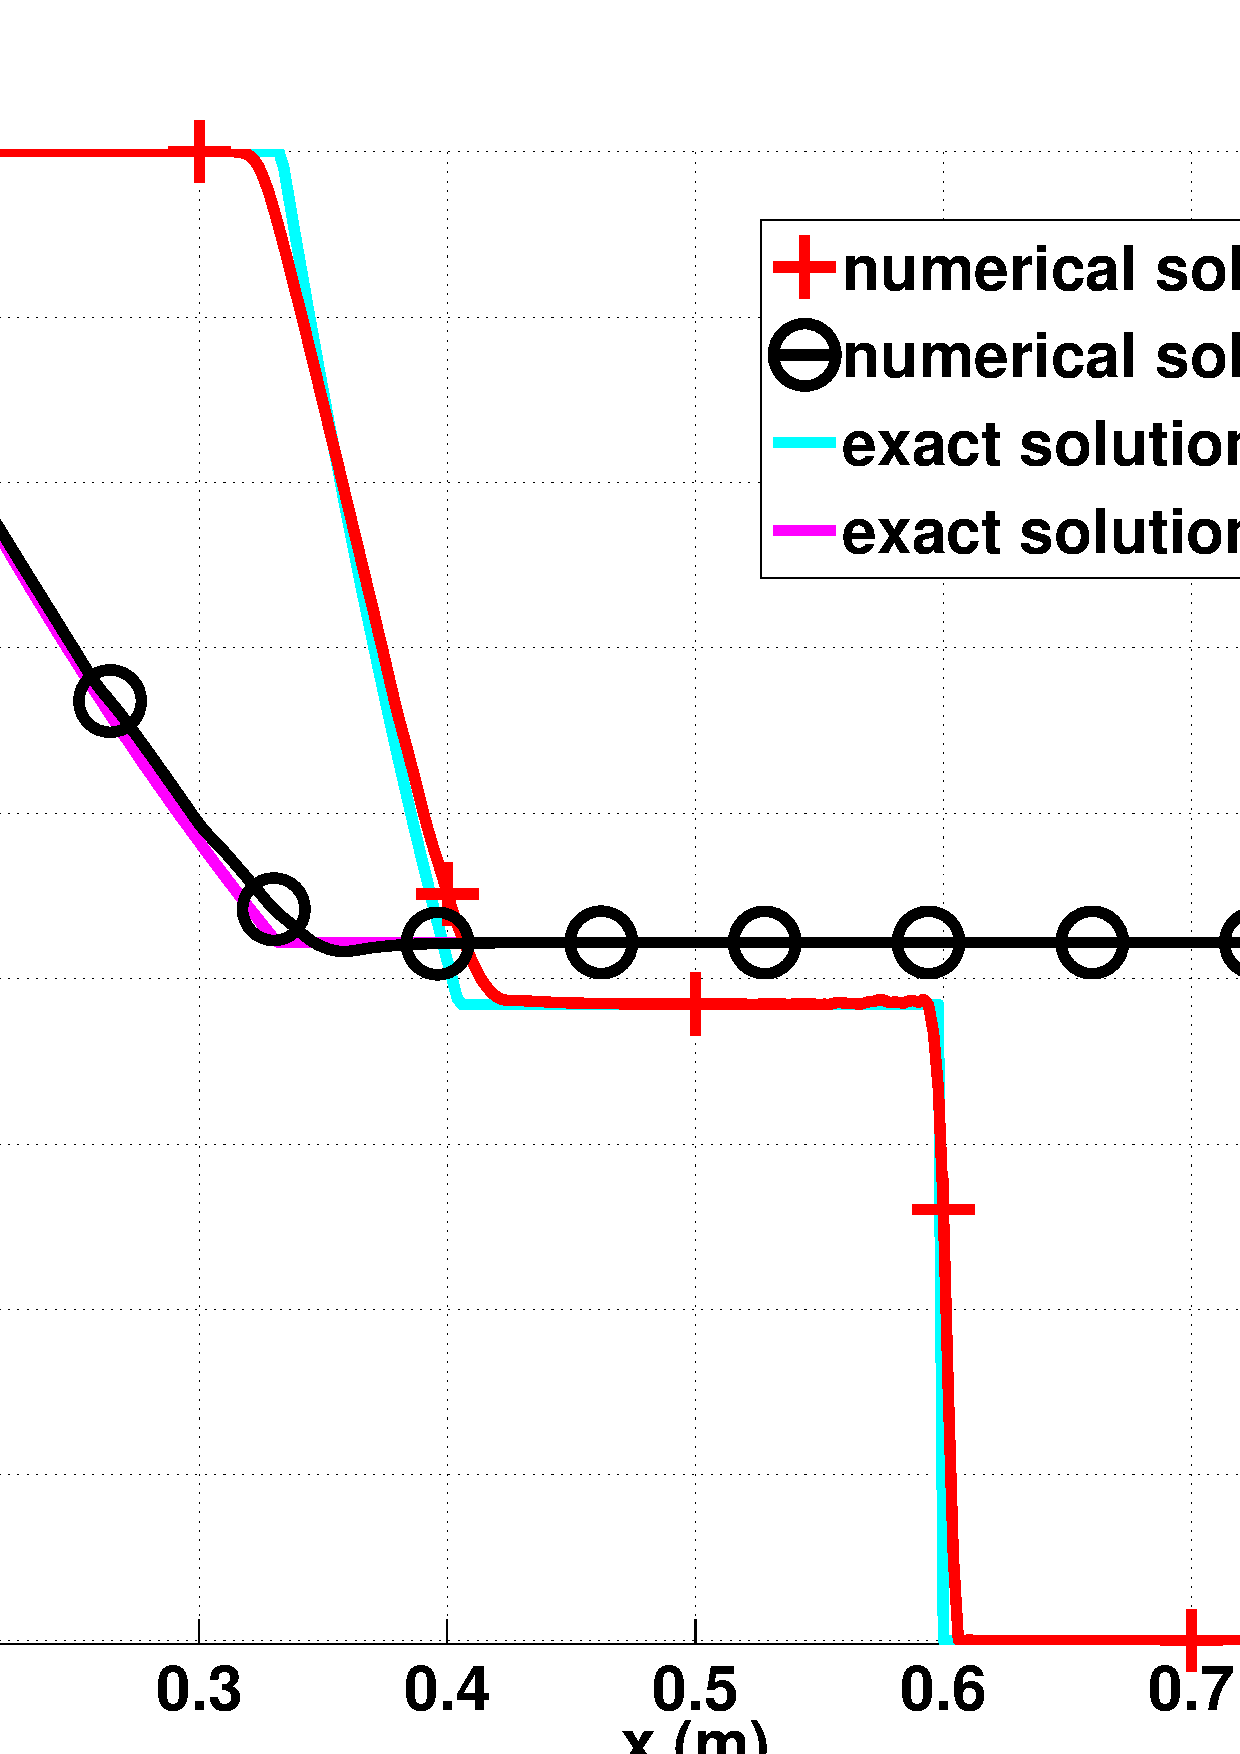
\includegraphics[width=\textwidth]{figures/SEM/two_phases_pressure.png}
                \caption{Pressure at $t=305$ $\mu s$}
        \end{subfigure}%
        \begin{subfigure}[b]{0.37\textwidth}
                \centering
                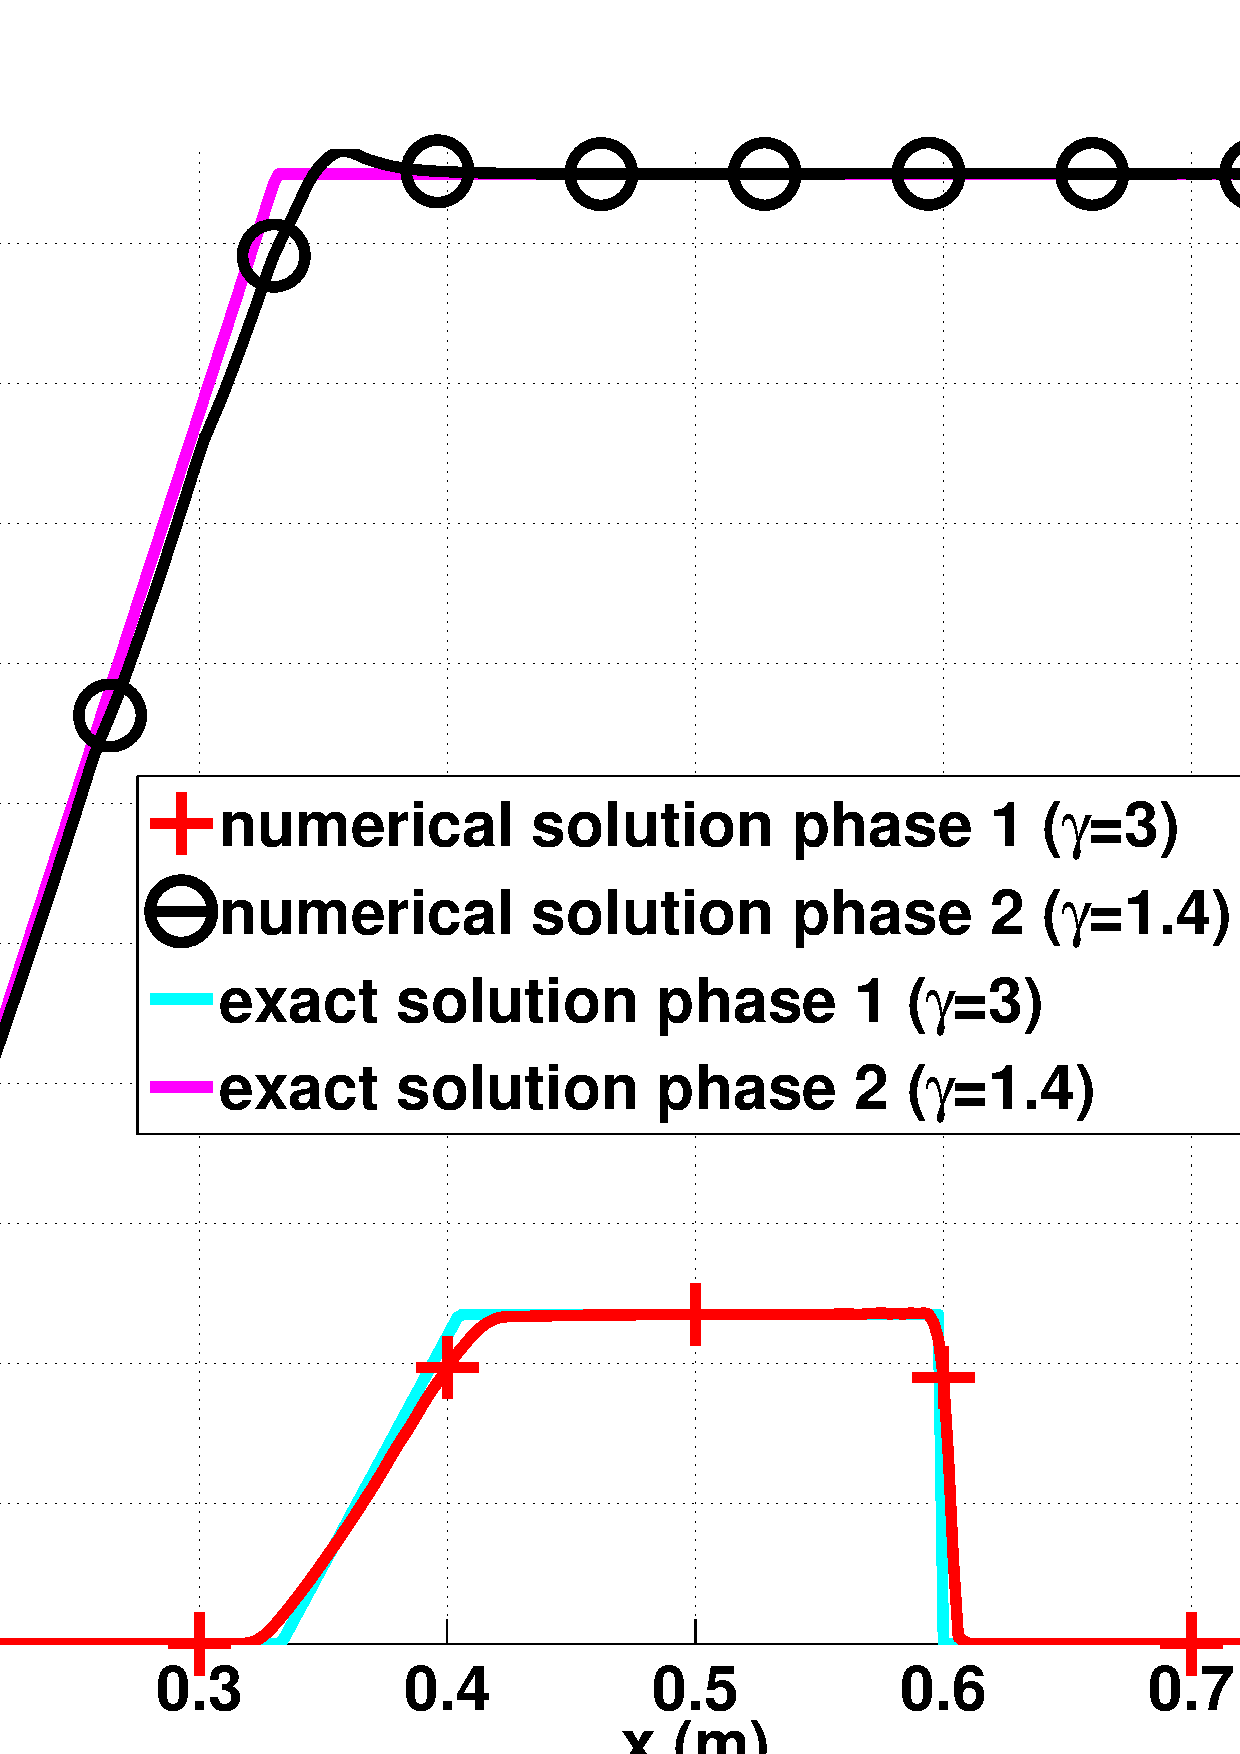
\includegraphics[width=\textwidth]{figures/SEM/two_phases_velocity.png}
                \caption{Velocity at $t=305$ $\mu s$}
        \end{subfigure}%

        \begin{subfigure}[b]{0.37\textwidth}
                \centering
                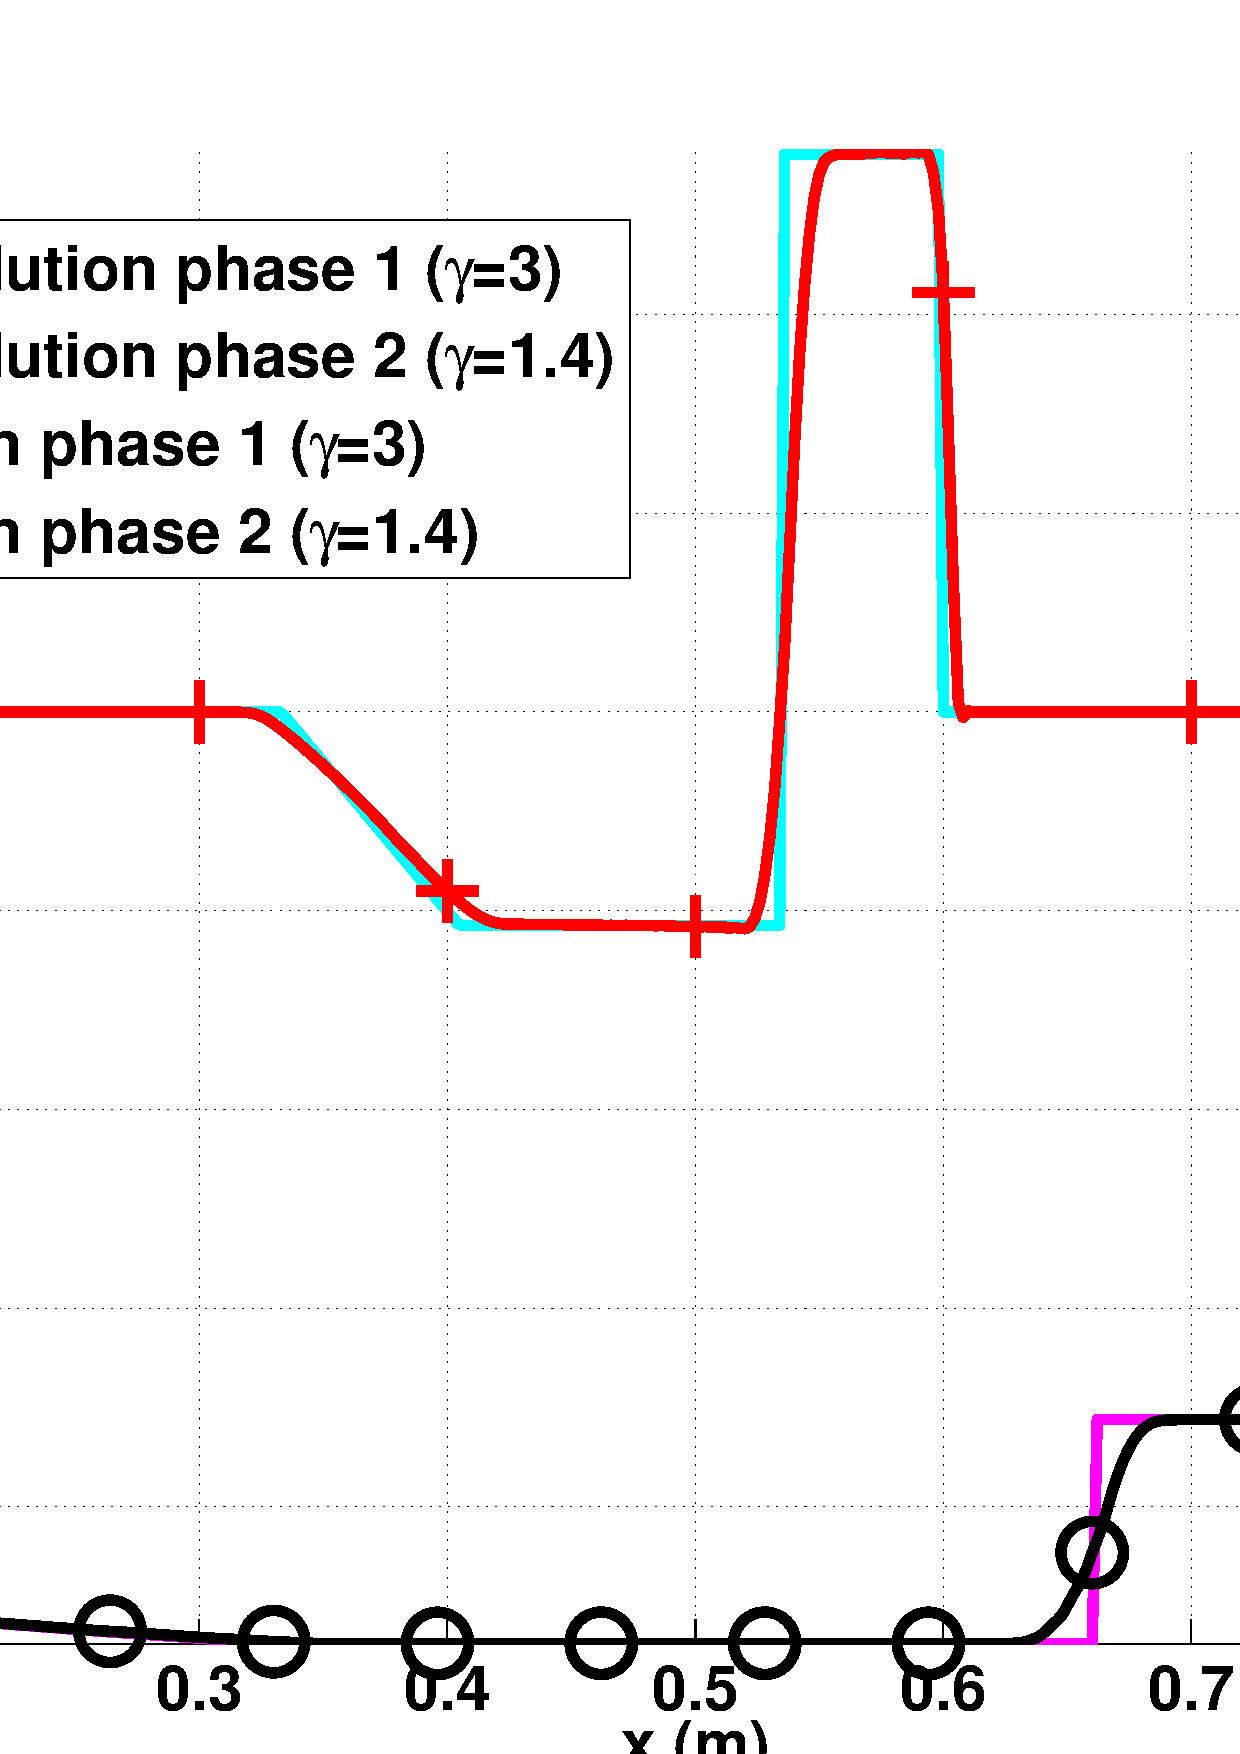
\includegraphics[width=\textwidth]{figures/SEM/two_phases_density.png}
                \caption{Density at $t=305$ $\mu s$}
        \end{subfigure}%
        \begin{subfigure}[b]{0.37\textwidth}
                \centering
                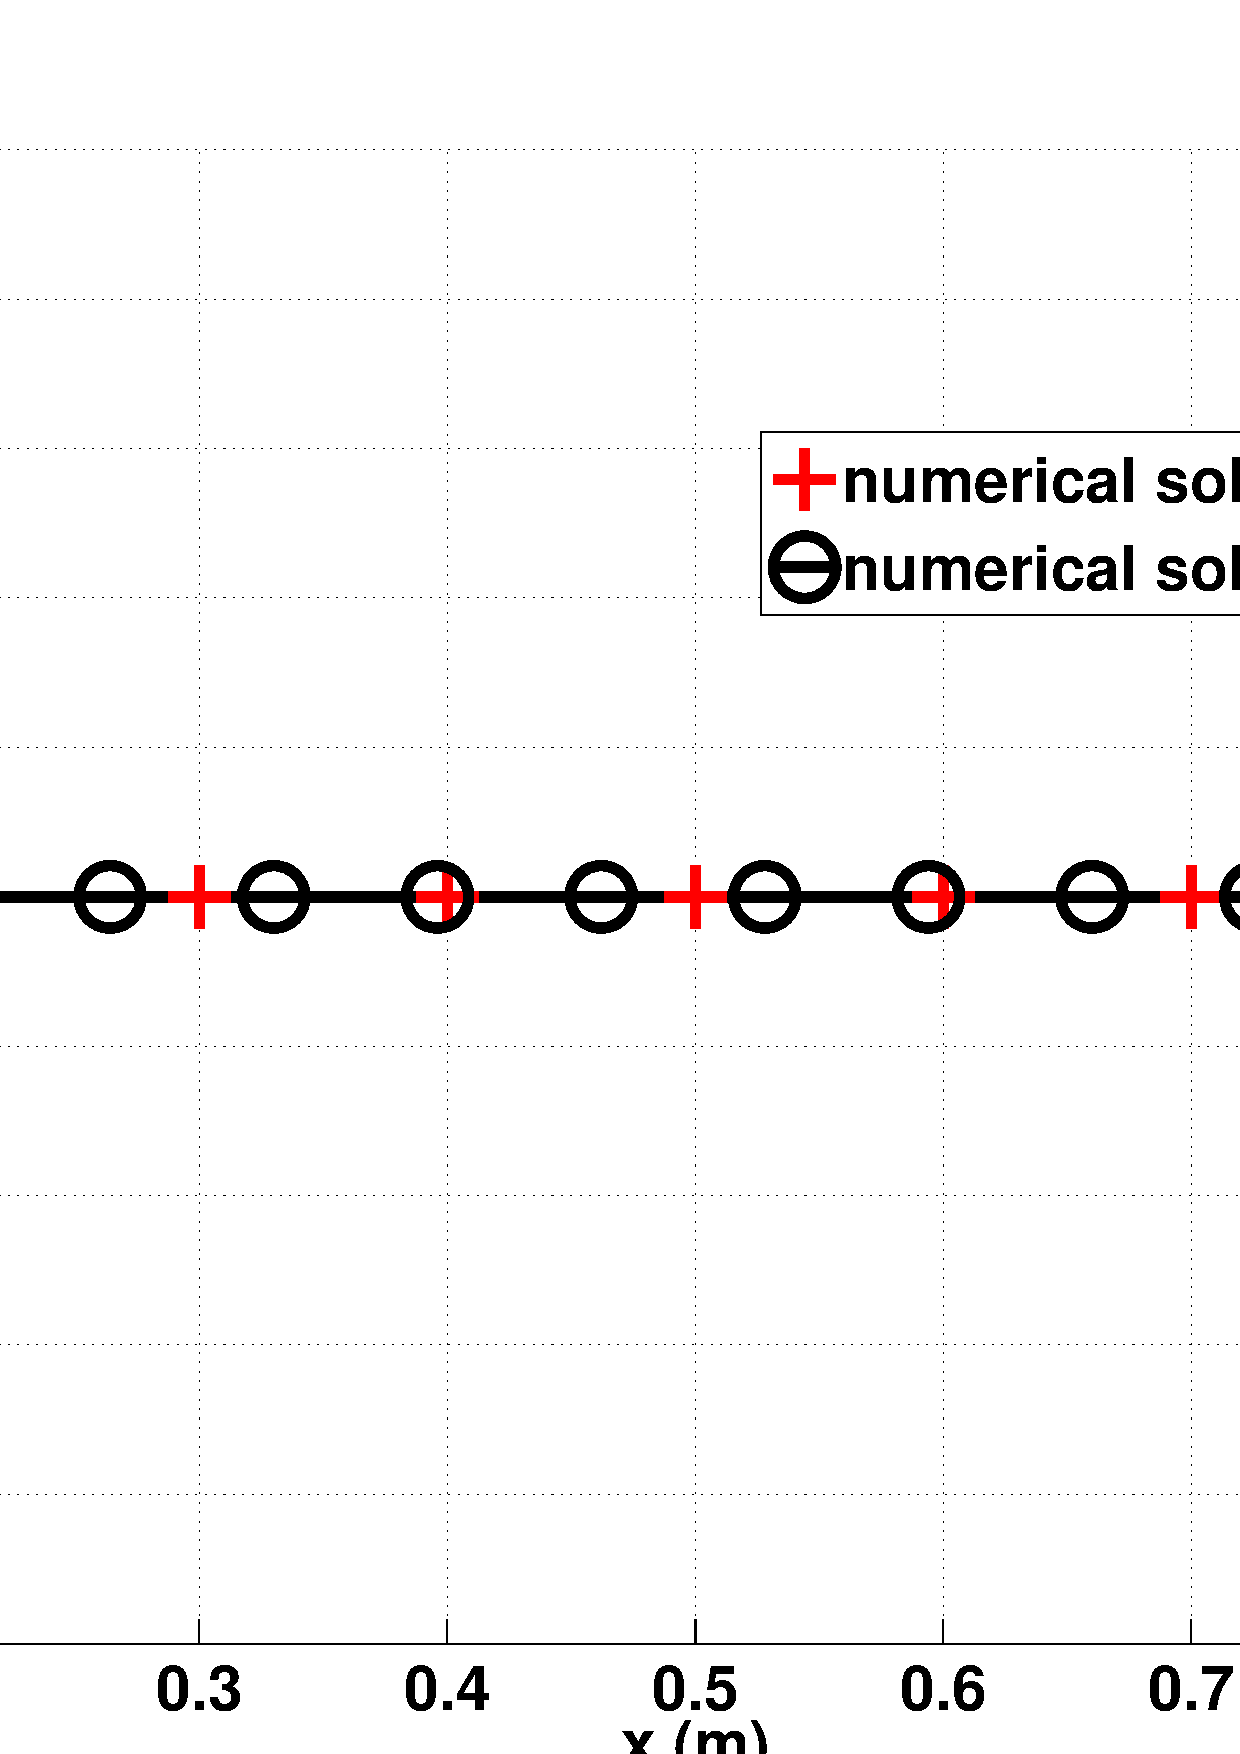
\includegraphics[width=\textwidth]{figures/SEM/two_phases_volume_fraction.png}
                \caption{Volume fraction at $t=305$ $\mu s$}
        \end{subfigure}%
\end{figure}
\end{frame}
%************************************************
\begin{frame}{$1$-D shock tube with two independent fluids}
\begin{figure}
        \begin{subfigure}[b]{0.37\textwidth}
                \centering
                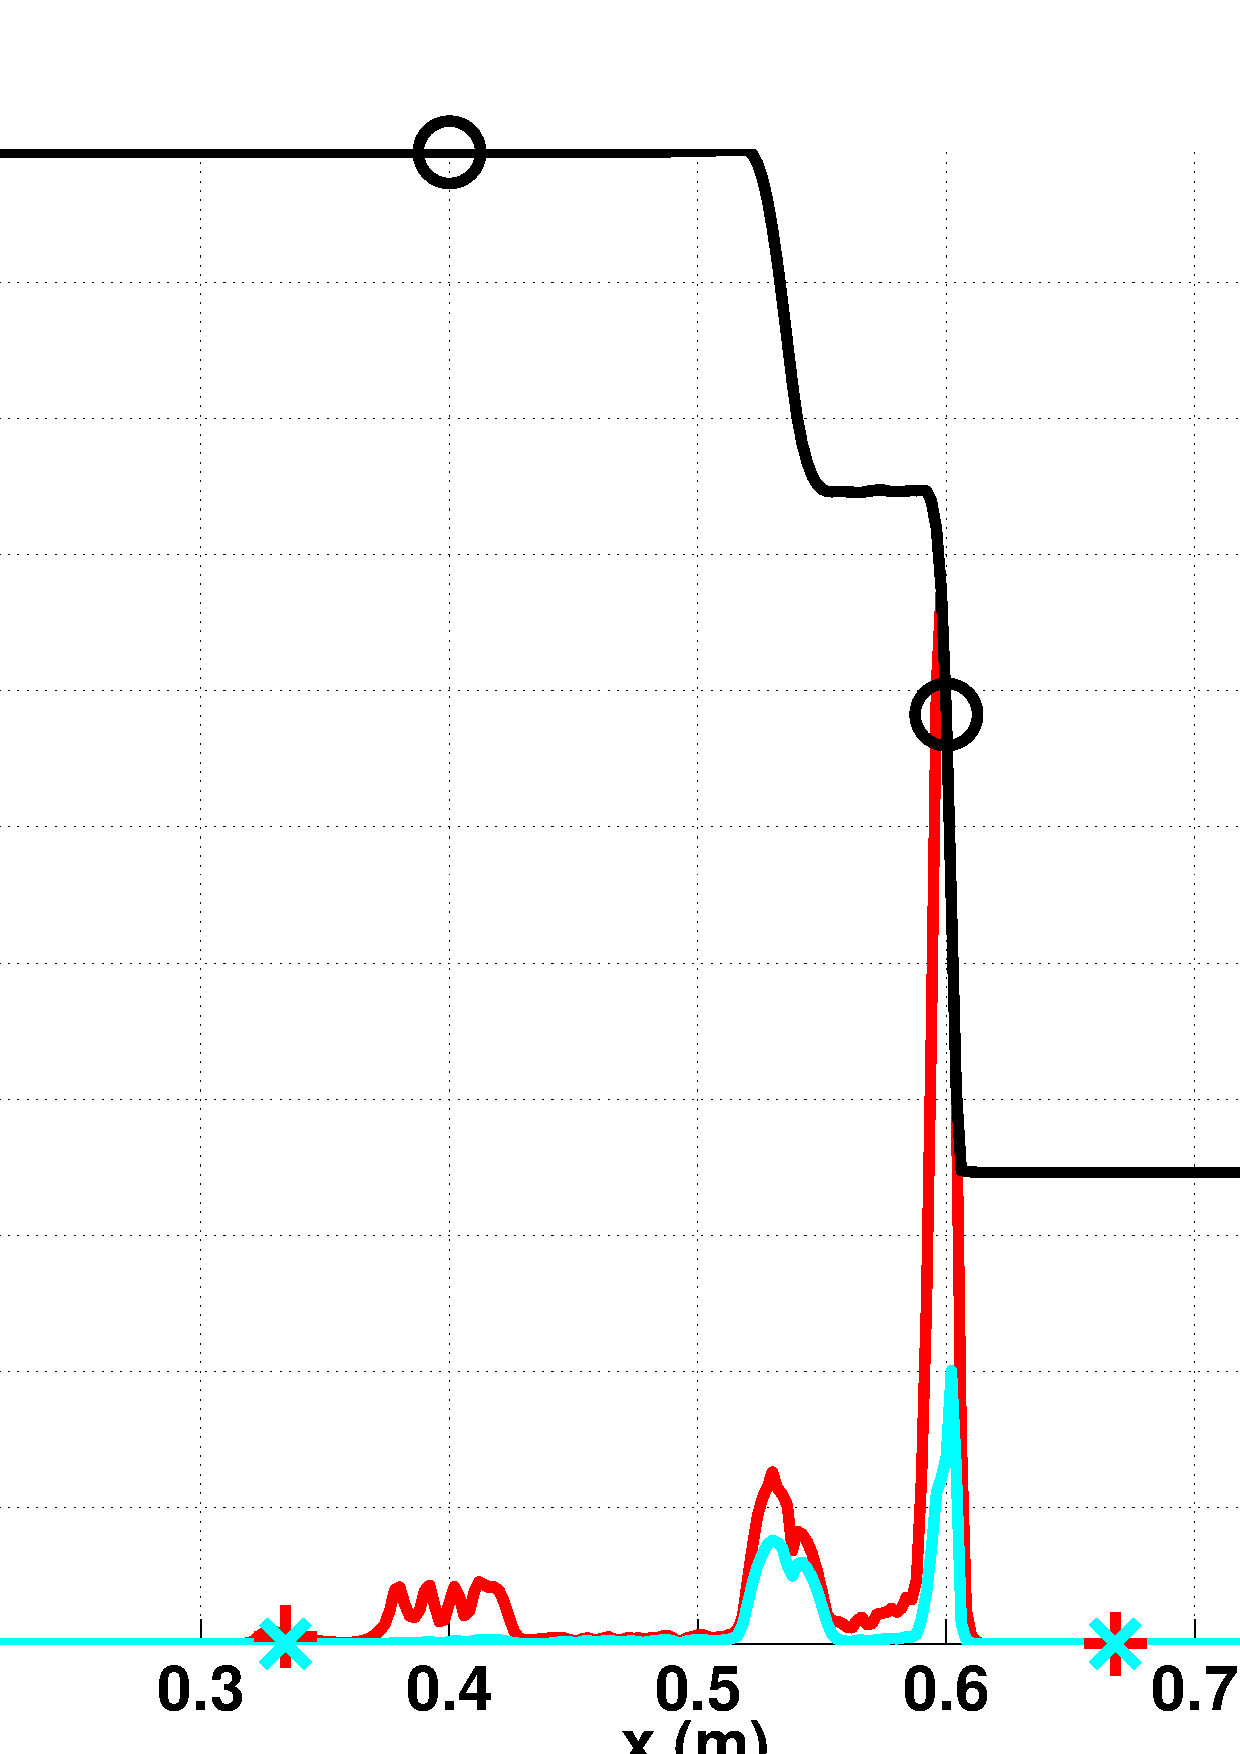
\includegraphics[width=\textwidth]{figures/SEM/two_phases_liquid_viscosity_kappa_mu.png}
                \caption{Viscosity coefficients phase $1$}
        \end{subfigure}%
        \begin{subfigure}[b]{0.37\textwidth}
                \centering
                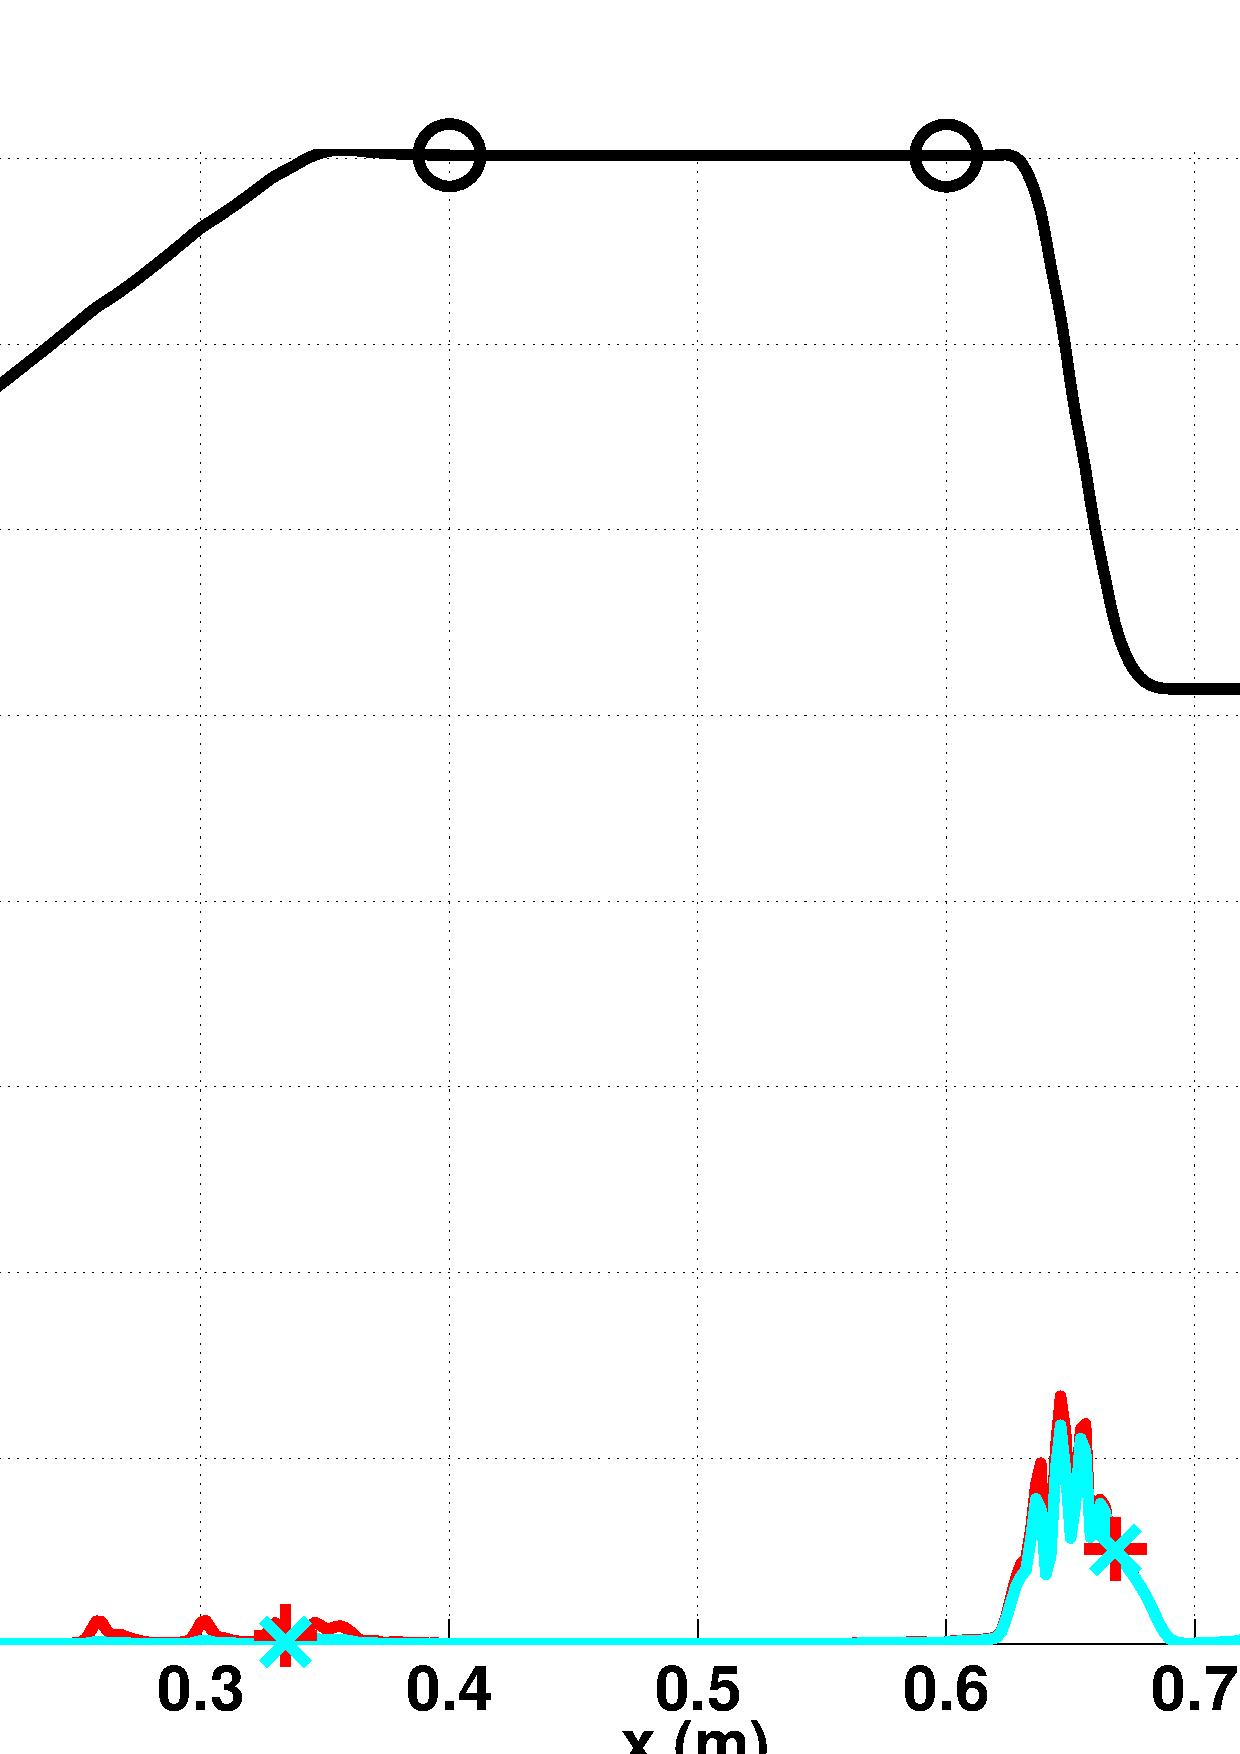
\includegraphics[width=\textwidth]{figures/SEM/two_phases_vapor_viscosity_kappa_mu.png}
                \caption{Viscosity coefficients phase $2$}
        \end{subfigure}%
\end{figure}
\begin{figure}[H]        
\centering
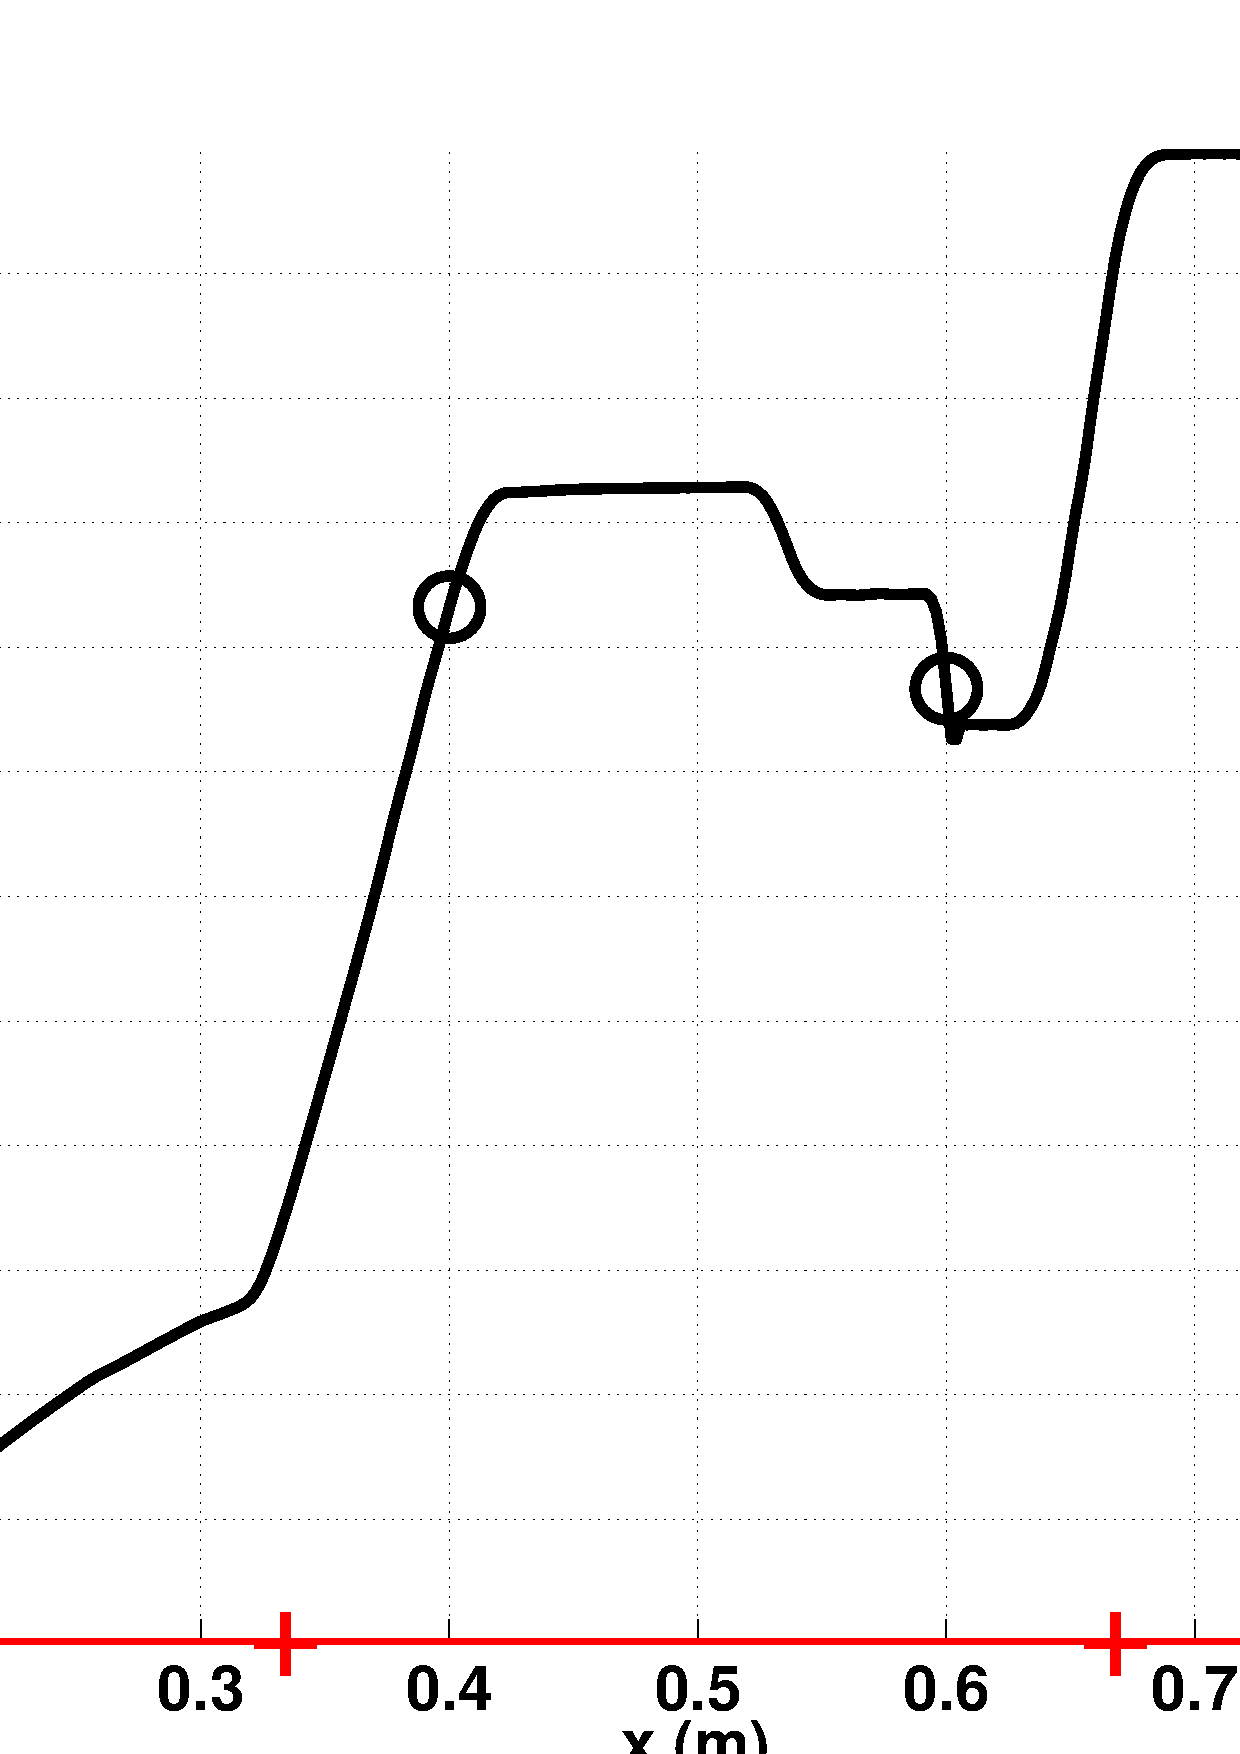
\includegraphics[width=0.37\textwidth]{figures/SEM/two_phases_liquid_beta.png}
\caption{Viscosity coefficients volume fraction}
\end{figure}
\end{frame}
%************************************************
\begin{frame}{$1$-D shock tube with infinite relaxation coefficients}
\begin{block}{}
\begin{itemize}
\setlength{\itemsep}{5pt}
\item same fluids, same initial conditions and same equations of state
\item relaxation parameters are turned on and computed with $A_{int,max} = 10^4 m^{-1}$
\begin{align}
\mu_p = \frac{A_{int}}{Z_1+Z_2} \nonumber \\
\lambda_u = \frac{\mu_P}{2} Z_1 Z_2 \nonumber \\
A_{int} = A_{int,max} \nonumber
\end{align}
\item volume fraction will vary because of the pressure relaxation term
\item NO exact solution available
\end{itemize}
\end{block}
Objective: verify that the volume fraction is correctly stabilized by the EVM
\end{frame}
%************************************************
\begin{frame}{$1$-D shock tube with infinite relaxation coefficients}
\begin{figure}
        \begin{subfigure}[b]{0.37\textwidth}
                \centering
                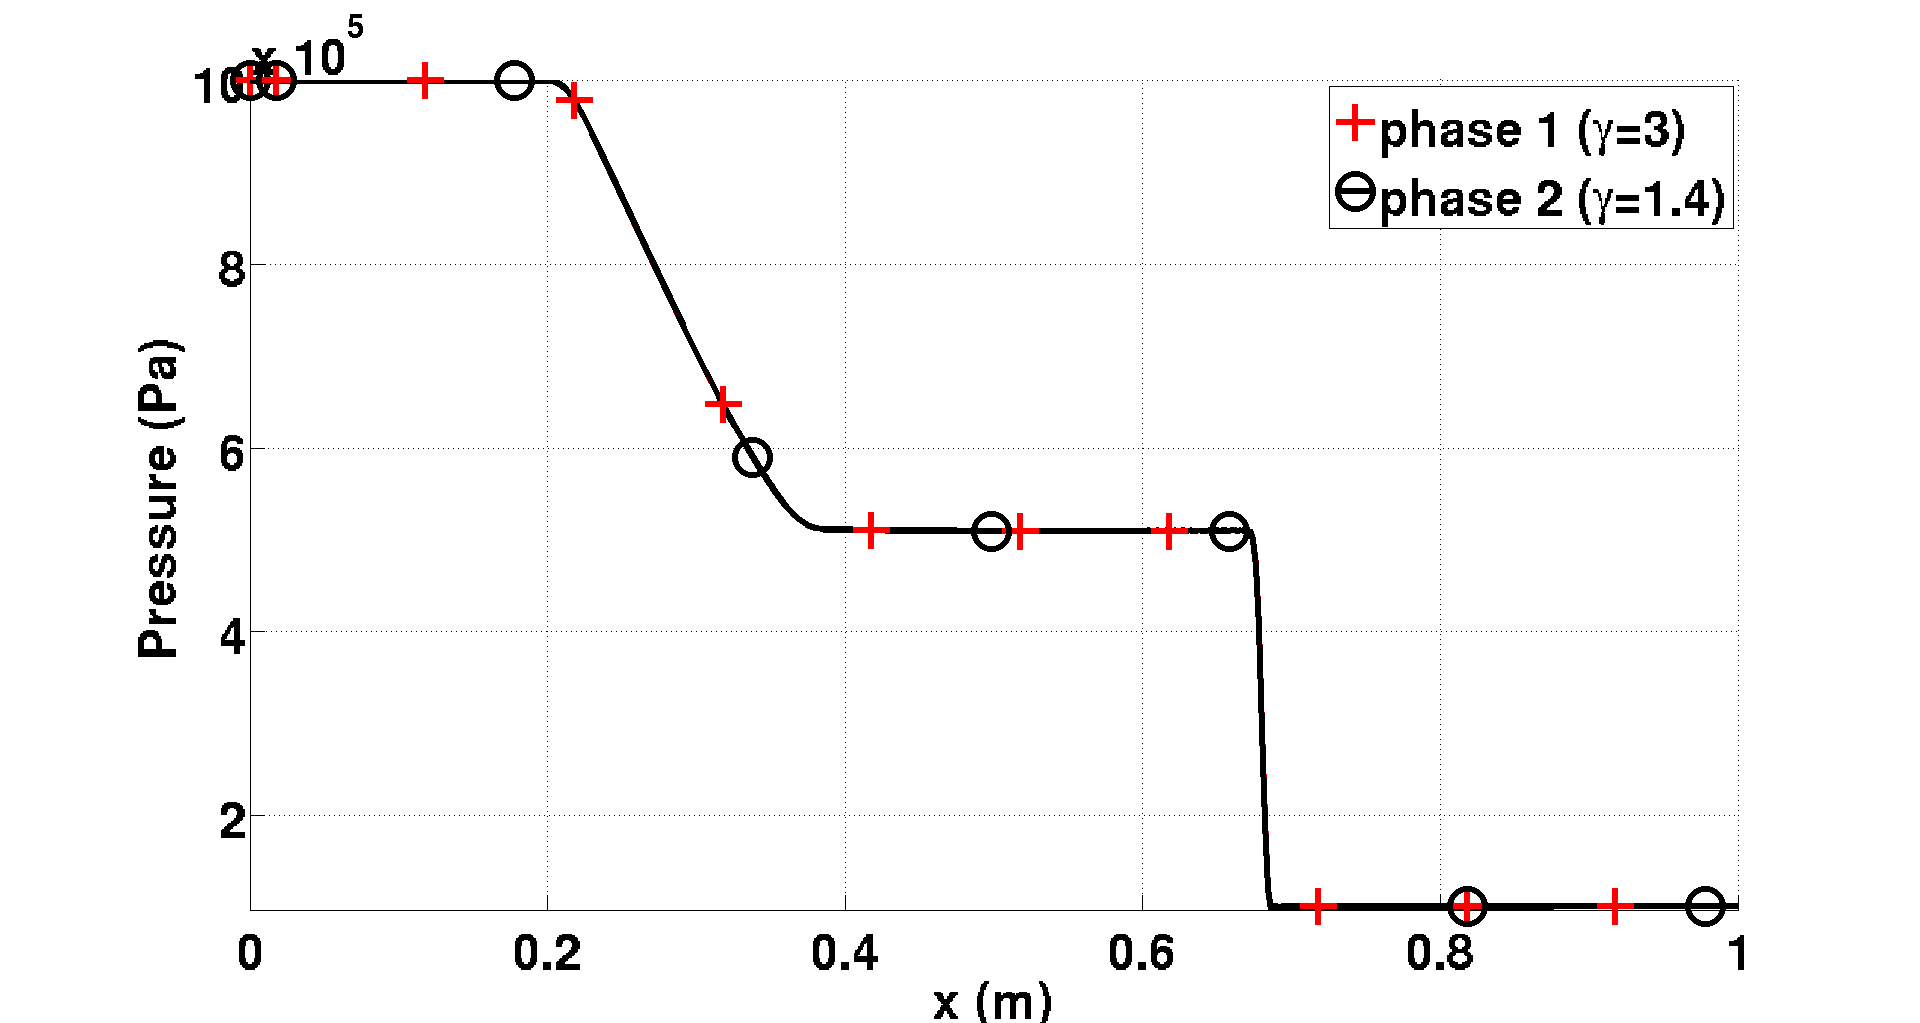
\includegraphics[width=\textwidth]{figures/SEM/relaxation_two_phases_pressure.png}
                \caption{Pressure at $t=305$ $\mu s$}
        \end{subfigure}%
        \begin{subfigure}[b]{0.37\textwidth}
                \centering
                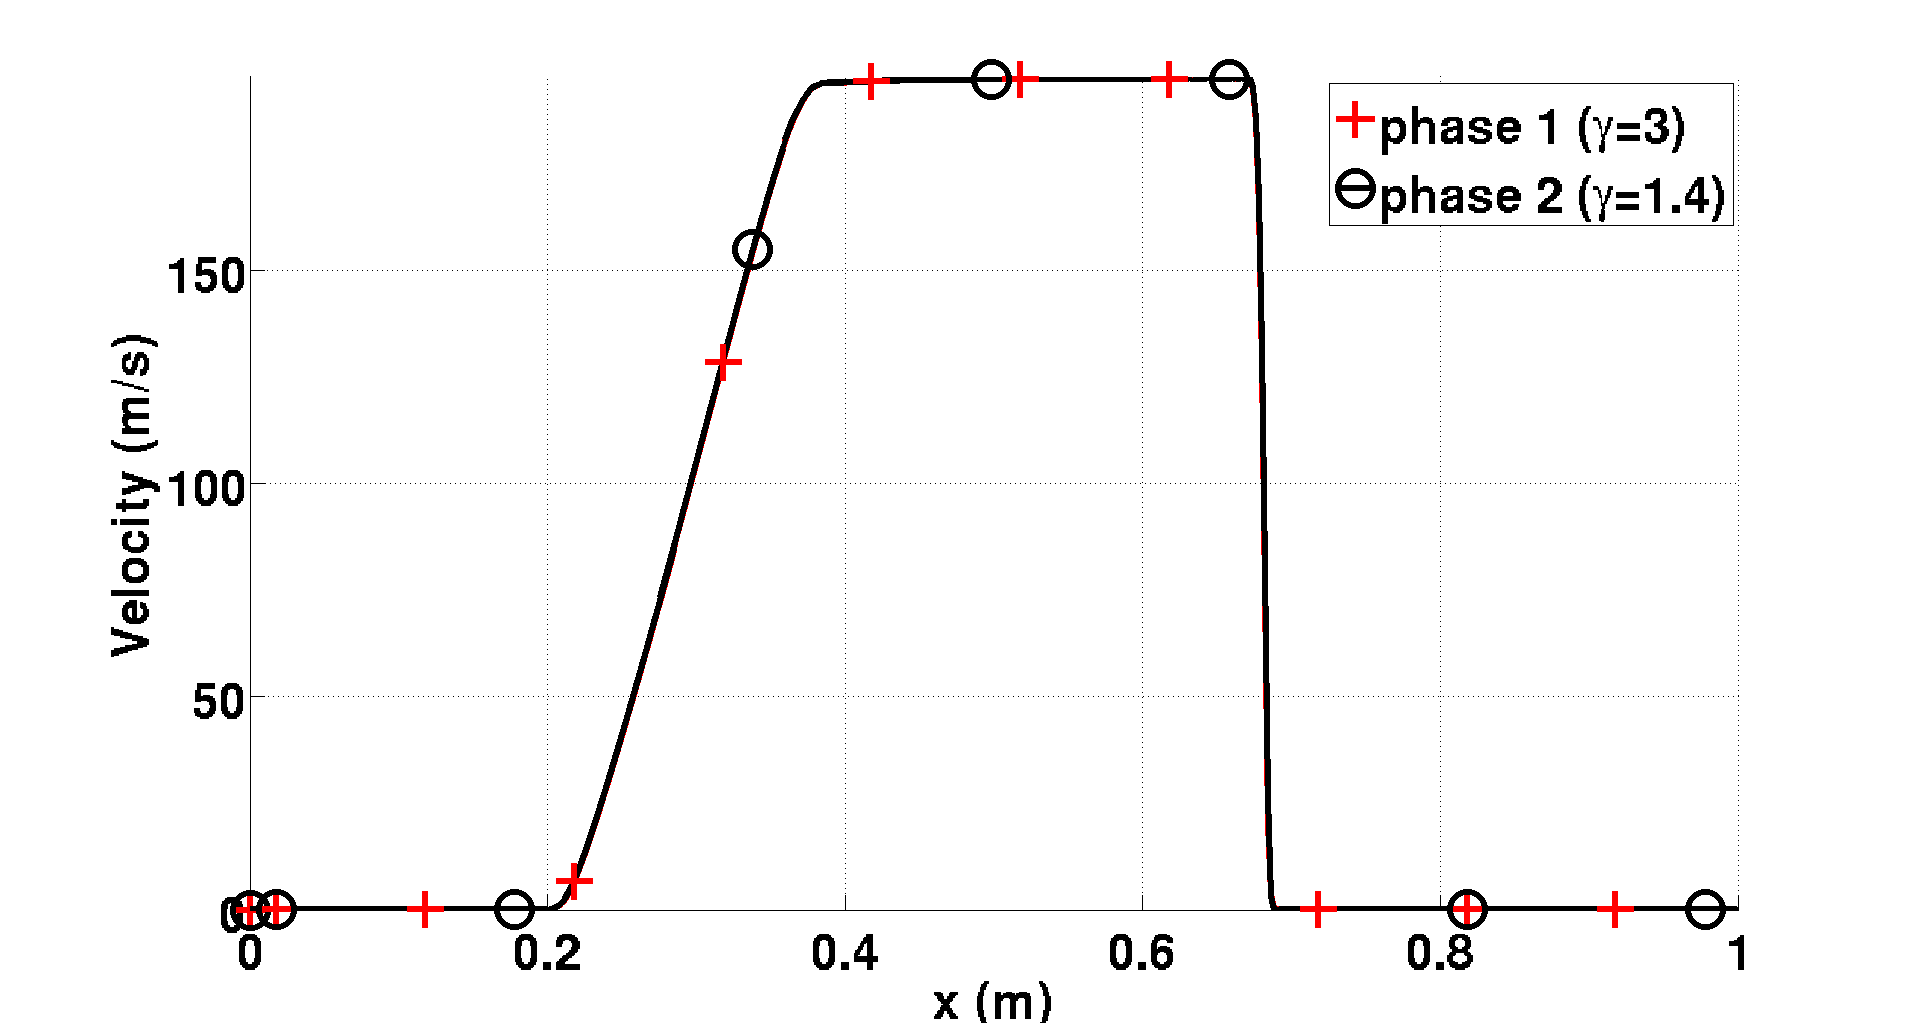
\includegraphics[width=\textwidth]{figures/SEM/relaxation_two_phases_velocity.png}
                \caption{Velocity at $t=305$ $\mu s$}
        \end{subfigure}%

        \begin{subfigure}[b]{0.37\textwidth}
                \centering
                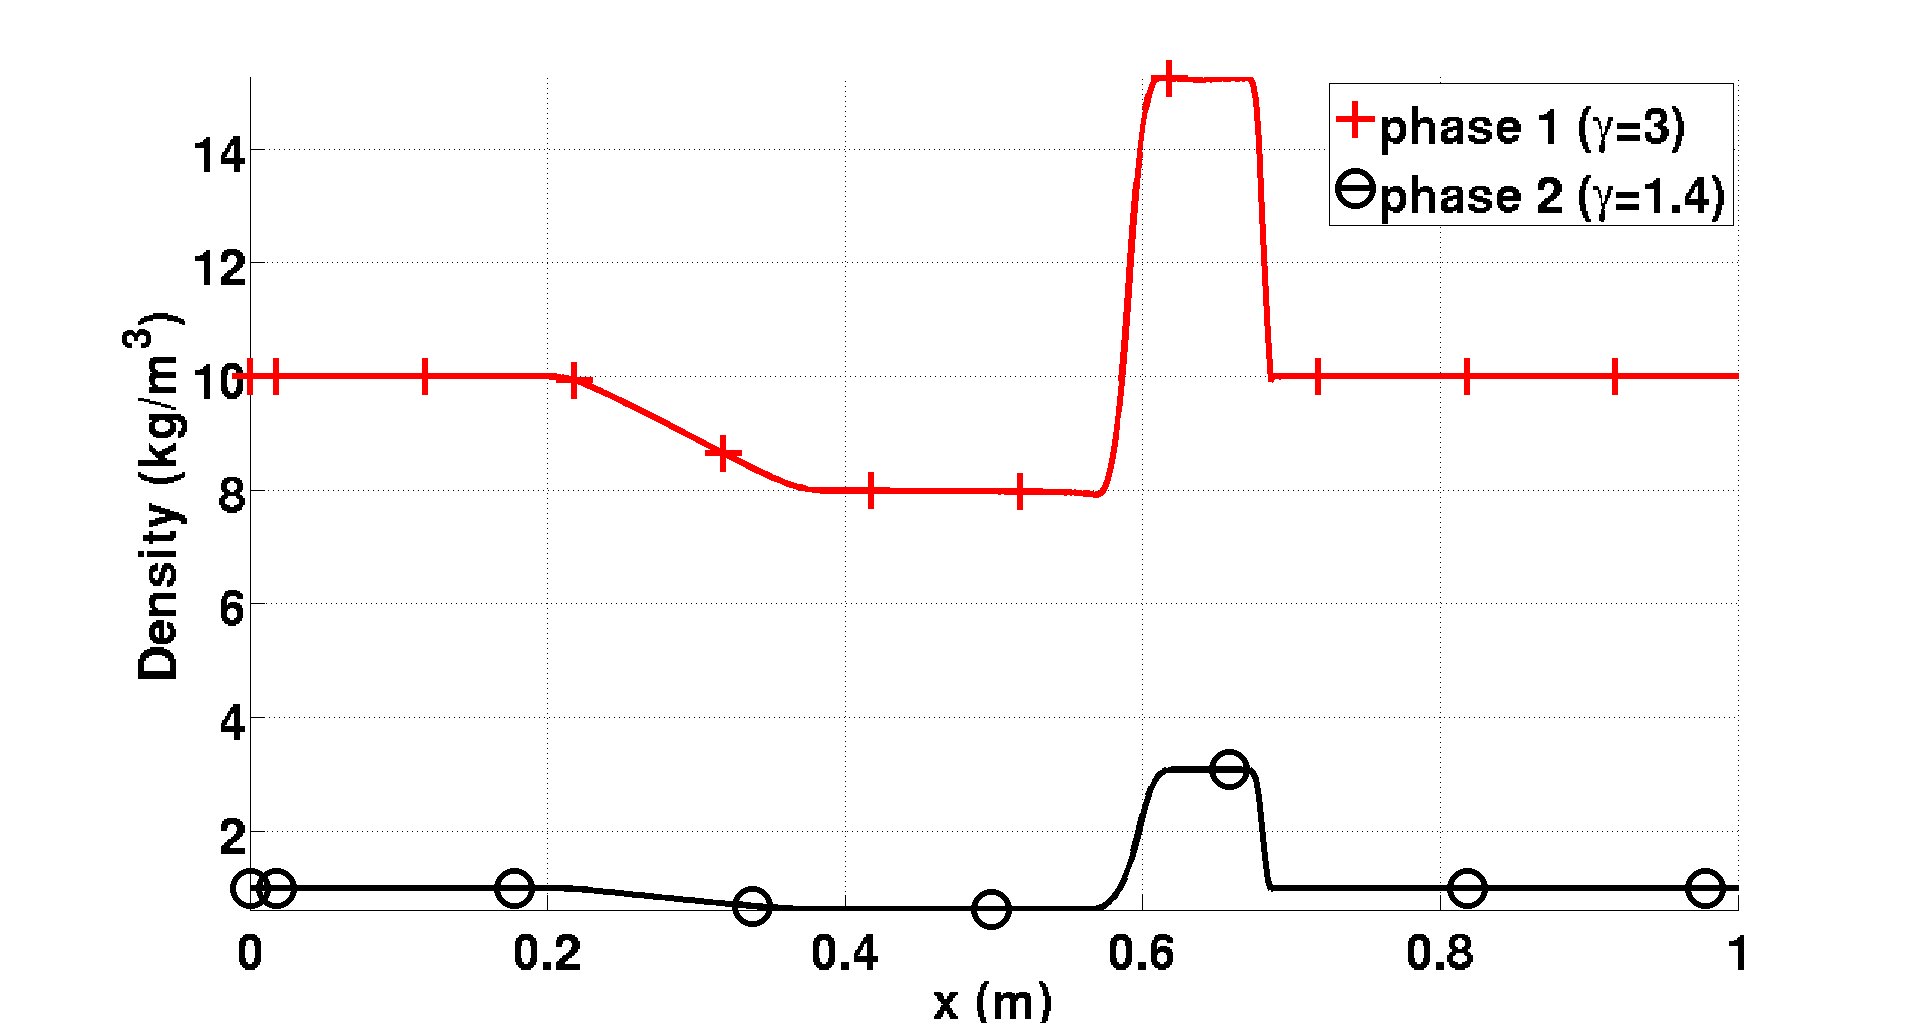
\includegraphics[width=\textwidth]{figures/SEM/relaxation_two_phases_density.png}
                \caption{Density at $t=305$ $\mu s$}
        \end{subfigure}%
        \begin{subfigure}[b]{0.37\textwidth}
                \centering
                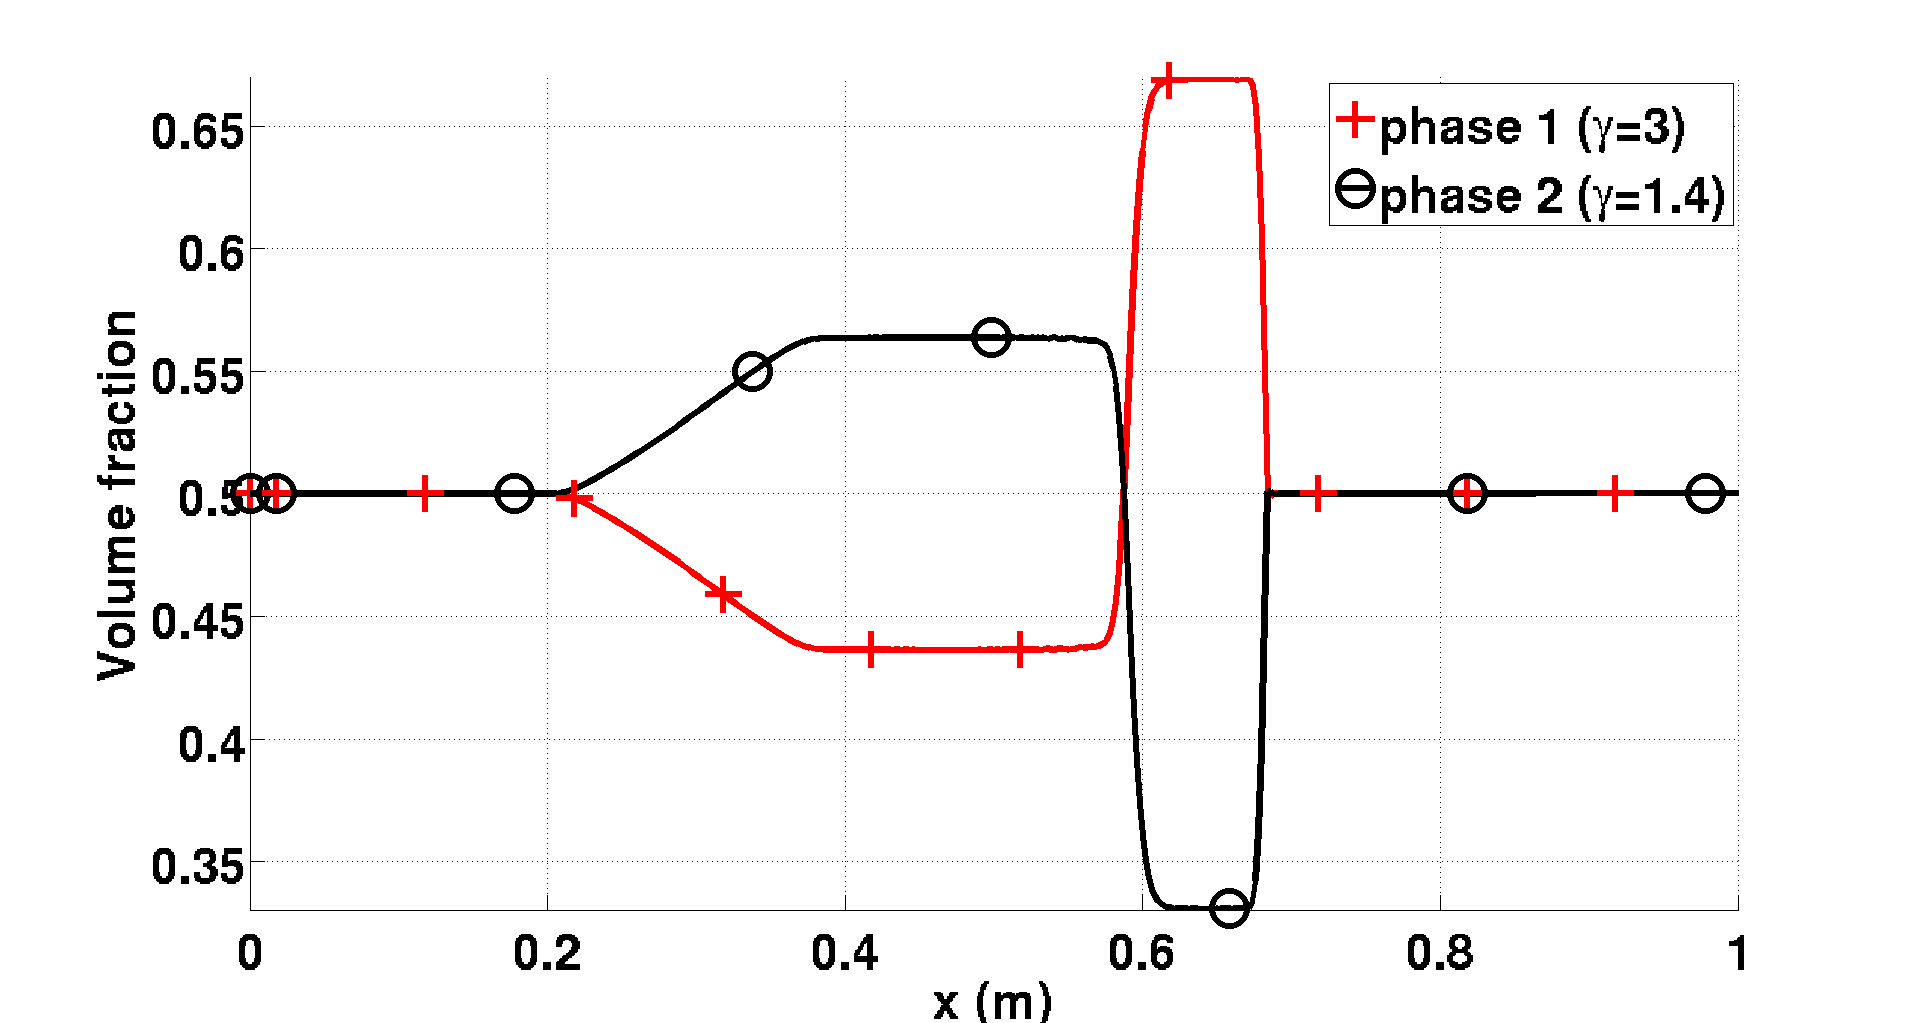
\includegraphics[width=\textwidth]{figures/SEM/relaxation_two_phases_volume_fraction.png}
                \caption{Volume fraction at $t=305$ $\mu s$}
        \end{subfigure}%
\end{figure}
\end{frame}
%************************************************
\begin{frame}{$1$-D shock tube with infinite relaxation coefficients}
\begin{figure}
        \begin{subfigure}[b]{0.37\textwidth}
                \centering
                \includegraphics[width=\textwidth]{figures/SEM/relaxation_two_phases_liquid_viscosity_kappa_mu.png}
                \caption{Viscosity coefficients phase $1$}
        \end{subfigure}%
        \begin{subfigure}[b]{0.37\textwidth}
                \centering
                \includegraphics[width=\textwidth]{figures/SEM/relaxation_two_phases_vapor_viscosity_kappa_mu.png}
                \caption{Viscosity coefficients phase $2$}
        \end{subfigure}%
\end{figure}
\begin{figure}[H]        
\centering
\includegraphics[width=0.37\textwidth]{figures/SEM/relaxation_two_phases_liquid_beta.png}
\caption{Viscosity coefficients volume fraction}
\end{figure}
\end{frame}

%%************************************************
\begin{frame}{Hydrostatic test}
Initially fully mixed phases ($\alpha=0.5$). Gravity separates phases (counter-current flow).
\begin{center}
\movie[width=6cm,height=4cm,showcontrols=true,externalviewer]{\includegraphics[width=6cm,height=4cm]{engr.pdf}}{hydrostatic-test-400-cells_3_8.avi} %%%% two-phase-hydrostatic.avi}
\end{center}
\end{frame}
%%************************************************

%%************************************************
\begin{frame}{Water hammer}
Water hammer, or hydraulic shock, is a pressure surge or wave caused when a fluid in motion is forced to stop or change direction abruptly.
\begin{center}
\movie[width=6cm,height=4cm,showcontrols=true,externalviewer]{\includegraphics[width=6cm,height=4cm]{engr.pdf}}{two-phase-WH.avi}
\end{center}
\end{frame}
%%************************************************

%************************************************
%************************************************
\section{Conclusions and future work}
%************************************************
%************************************************

%************************************************
\begin{frame}{Conclusions and future work}
\begin{block}{Euler equations}
\begin{itemize}
\item removed the need to have an entropy function
\item extended the EVM to low-Mach flows through a low-Mach asymptotic analysis 
\item validated our approach with $1$ and $2$-D simulations and convergence tests
\item used as a numerical method in RELAP-7
%\item applied the EVM with the Stiffened Gas equation of state (not shown)
\end{itemize}
\end{block}
\begin{block}{The seven-equation two-phase flow model (SEM)}
\begin{itemize}
\item derived a viscous regularization for the SEM
\item defined the viscosity coefficients using the same methodology as for single-phase flow equation
\item our approach was validated by $1$-D results
\item used as a numerical method in RELAP-7
\end{itemize}
\end{block}
\begin{block}{MOOSE/RELAP-7}
Fully  implicit temporal discretization with {\it continuous} FEM through MOOSE\\
Used in the next-gen nuclear reactor safety code RELAP-7
\end{block}
\end{frame}

\end{document}

\begin{frame}{The $1$-D grey Radiation-Hydrodynamic equations (GRHD):}

\begin{block}{GRHD system of equations (before viscous regularization):}
\begin{align}
%\left\{
%\begin{array}{lll}
&\partial_t \left( \rho \right) + \partial_x\left( \rho u \right) = 0 \nonumber\\
&\partial_t \left( \rho u\right) + \partial_x \left(\rho u^2 + P  \right) = {\color{blue}-\partial_x \left(\frac{\epsilon}{3}\right)} \nonumber\\
&\partial_t \left( \rho E\right) + \partial_x \left[ u \left( \rho E + P \right) \right] = {\color{blue}-\frac{u}{3} \partial_x \epsilon - \sigma_a c \left( a T^4 - \epsilon \right)} \nonumber\\
&\partial_t \epsilon + \frac{4}{3} \partial_x \left( u \epsilon \right) = {\color{blue}\frac{u}{3} \partial_x \epsilon} + {\color{magenta}\partial_x \left( \frac{c}{3 \sigma_t} \partial_x \epsilon \right)} + {\color{blue}\sigma_a c \left( a T^4 - \epsilon \right)} \nonumber
%\end{array}
%\right. 
\nonumber
\end{align}
\end{block}

%\begin{block}{A few remarks:}
%\begin{itemize}
%\setlength{\itemsep}{10pt}
%\item Relaxation term in the energy and radiation equations: ${\color{blue}\sigma_a c \left( a T^4 - \epsilon \right)}$.% behaves like a diffusion term when $\sigma_a \to \infty$ \cite{ShiJin}.
%\item Diffusion term: ${\color{magenta}\partial_x \left( \frac{c}{3 \sigma_t} \partial_x \epsilon \right)}$.
%\item The above system of equations is NOT hyperbolic, and yet ...
%\end{itemize}
%\end{block}

%\begin{block}{Other applications where we have applied the entropy-viscosity technique}
%\begin{itemize}
%\item Shallow-water equations for flooding and inundations
%\end{itemize}
%\end{block}

\end{frame}

%\end{document}
%------------------------------------------------------
%\begin{frame}{Steady-state solution for Mach $1.05$ (continuous FEM)}
%
%\begin{figure}[H]
%\centering
%\subfigure[Temperatures]{
%\includegraphics[width=0.3\textwidth]{figures/Mach_1p05_nel_500_temperature.png}
%}
%\subfigure[Material density]{
%\includegraphics[width=0.3\textwidth]{figures/Mach_1p05_nel_500_density.png}
%}
%\subfigure[Viscosity coefficient]{
%\includegraphics[width=0.3\textwidth]{figures/Mach_1p05_nel_500_viscosity.png}
%}
%\end{figure}
%
%\end{frame}
%************************************************

\begin{frame}{Steady-state solution for Mach $2$ (continuous FEM)}

\begin{figure}[H]
\centering
   \begin{subfigure}[b]{0.37\textwidth}
   \includegraphics[width=\textwidth]{figures/Mach_2_nel_2000_temperature.png}
   \caption{Temperatures}
   \end{subfigure}
   \begin{subfigure}[b]{0.37\textwidth}
   \includegraphics[width=\textwidth]{figures/Mach_2_nel_2000_density.png}
   \caption{Material density}
   \end{subfigure}
   \begin{subfigure}[b]{0.37\textwidth}
   \includegraphics[width=\textwidth]{figures/Mach_2_nel_2000_viscosity.png}
   \caption{Viscosity coefficient}
   \end{subfigure}
\end{figure}

\end{frame}
%************************************************
\begin{frame}{Steady-state solution for Mach $5$ (continuous FEM)}

\begin{figure}[H]
\centering
   \begin{subfigure}[b]{0.37\textwidth}
   \includegraphics[width=\textwidth]{figures/Mach_5_nel_1000_temperature.png}
   \caption{Temperatures}
   \end{subfigure}
   \begin{subfigure}[b]{0.37\textwidth}
   \includegraphics[width=\textwidth]{figures/Mach_5_nel_2000_density.png}
   \caption{Material density}
   \end{subfigure}
   \begin{subfigure}[b]{0.37\textwidth}
   \includegraphics[width=\textwidth]{figures/Mach_5_nel_2000_viscosity.png}
   \caption{Viscosity coefficient}
   \end{subfigure}
   \begin{subfigure}[b]{0.37\textwidth}
   \includegraphics[width=\textwidth]{figures/Mach_5_comparison.png}
   \caption{Zoom at the Z spike}
   \end{subfigure}
\end{figure}


\end{frame}
%************************************************
\begin{frame}{Steady-state solution for Mach $50$ (continuous FEM)}

\begin{figure}[H]
\centering
   \begin{subfigure}[b]{0.37\textwidth}
   \includegraphics[width=\textwidth]{figures/Mach_50_nel_1000_temperature.png}
   \caption{Temperatures}
   \end{subfigure}
   \begin{subfigure}[b]{0.37\textwidth}
   \includegraphics[width=\textwidth]{figures/Mach_50_nel_1000_density.png}
   \caption{Material density}
   \end{subfigure}
   \begin{subfigure}[b]{0.37\textwidth}
   \includegraphics[width=\textwidth]{figures/Mach_50_nel_1000_viscosity.png}
   \caption{Viscosity coefficient}
   \end{subfigure}
\end{figure}

\end{frame}



%%************************************************
\begin{frame}{}
\label{lastslide}
\centering
Thank you 

\begin{figure}
	\centering
	\includegraphics[scale=0.33]{./crunching.png}
\end{figure}

\end{frame}
%%************************************************

%%%%%%%%%%%%%%%%%%%%%%%%%%%%%%%%%%%%%%%%%%%%%%%%%%%%%%%%%%%%%%%%%%%%%%%%%%%%%%%%
%%%%%%%%%%%%%%%%%%%%%%%%%%%%%%%%%%%%%%%%%%%%%%%%%%%%%%%%%%%%%%%%%%%%%%%%%%%%%%%%
%%%%%%%%%%%%%%%%%%%%%%%%%%%%%%%%%%%%%%%%%%%%%%%%%%%%%%%%%%%%%%%%%%%%%%%%%%%%%%%%
%%%%%%%%%%%%%%%%%%%%%%%%%%%%%%%%%%%%%%%%%%%%%%%%%%%%%%%%%%%%%%%%%%%%%%%%%%%%%%%%
%%%%%%%%%%%%%%%%%%%%%%%%%%%%%%%%%%%%%%%%%%%%%%%%%%%%%%%%%%%%%%%%%%%%%%%%%%%%%%%%
%%%%%%%%%%%%%%%%%%%%%%%%%%%%%%%%%%%%%%%%%%%%%%%%%%%%%%%%%%%%%%%%%%%%%%%%%%%%%%%%
%%%%%%%%%%%%%%%%%%%%%%%%%%%%%%%%%%%%%%%%%%%%%%%%%%%%%%%%%%%%%%%%%%%%%%%%%%%%%%%%
%%%%%%%%%%%%%%%%%%%%%%%%%%%%%%%%%%%%%%%%%%%%%%%%%%%%%%%%%%%%%%%%%%%%%%%%%%%%%%%%
%%%%%%%%%%%%%%%%%%%%%%%%%%%%%%%%%%%%%%%%%%%%%%%%%%%%%%%%%%%%%%%%%%%%%%%%%%%%%%%%
%%************************************************
\begin{frame}{}
\begin{center}
$1$-D Euler equations numerical results
\end{center}
\end{frame}
%%************************************************
\begin{frame}{Derivation of the entropy residual as a function of $\rho$, $P$, and $c$}
%
\vspace{-2mm}
%
\begin{block}{}
\begin{equation*}
\resi(\vec{r},t) = \partial_t s (\vec{r},t) + \vec{u} \cdot \grad s (\vec{r},t) = s_e  \matder{e} + s_{\rho}  \matder{\rho} 
\end{equation*}
\end{block}
%
%
\vspace{-2mm}
%
\begin{block}{}
\begin{eqnarray*}
\resi(\vec{r},t) &=&  s_e e_P \matder{P} + ( s_e e_{\rho} + s_{\rho} ) \matder{\rho} 
= s_e e_P \left( \matder{P} + \frac{1}{s_e e_P} ( s_e e_{\rho} + s_{\rho} )  \matder{\rho}\right) \\
&=& s_e e_P \left( \matder{P} + ( \frac{e_{\rho}}{e_P} + \frac{s_{\rho}}{s_e e_P} )  \matder{\rho} \right) \,.
\end{eqnarray*}
\end{block}
%
%
\vspace{-2mm}
%
\begin{block}{}
\begin{equation*}
c^2 := \left. \frac{\partial P}{\partial \rho} \right|_{s=cst} = P_{\rho} - \frac{s_{\rho}}{s_e} P_e   \, .
\end{equation*}
\end{block}
%
%
\vspace{-2mm}
%
\begin{block}{}
\begin{equation*}
P_e = \frac{1}{e_P} \text{ and } P_{\rho} = -\frac{e_{\rho}}{e_P}  \, .
\end{equation*}
%
\begin{equation*}
\resi(\vec{r},t) := \partial_t s + \vec{u} \cdot \grad s = \matder{s} = \frac{s_e}{P_e} \left( \underbrace{\matder{P} - c^2 \matder{\rho} }_{\resinew(\vec{r},t)} \right) \, .
\end{equation*} 
\end{block}

\end{frame}
%%************************************************
\begin{frame}{Entropy residual with viscous regularization for Euler equations}
\begin{block}{Entropy equation}
\begin{align}
A \rho \left( \partial_t s + \mbold{u} \cdot \div s \right) = \div \left( \rho A \kappa \grad s \right) - A \kappa \rho \mathbf{Q} + A s_e \mu \grad^s \mbold{u} : \grad \mbold{u} \nonumber
\end{align}
\end{block}
%
\begin{block}{Matrix definition}
\begin{eqnarray}
\mathbf{Q} &=& X^t \Sigma X \nonumber \\
\text{with } X &=& \begin{bmatrix}
\grad \rho \\
\grad e 
\end{bmatrix}
\text{and } \Sigma = \begin{bmatrix}
       \partial_{\rho} (\rho^2 \partial_{\rho} s) & \partial_{\rho,e} s  \\[0.3em]
       \partial_{\rho,e} s & \partial_{e,e} s           \\[0.3em]
     \end{bmatrix} \nonumber 
\end{eqnarray}
The matrix $Q$ is negative definite if and only if $-s$ is convex with respect to $e$ and $\rho^{-1}$.
\end{block}
\end{frame}
%%************************************************
\begin{frame}{}
\begin{block}{A normalization function for $\mu_e$}
\begin{equation}
\mu_e = h^2 \frac{\max \left( |\resinew|, J_P \right)}{\norm_P^\mu} \nonumber
\end{equation}
\begin{equation}
\norm_P^\mu = (1 - b(M) ) \rho c^2 + b(M) \rho || \vec{u} ||^2 \text{ where } \lim_{M\to 0} b = 0\nonumber
\end{equation}
\end{block}
\begin{block}{Example}
\begin{equation}
b(M) = \frac{\tanh (a(M-M_{threshold})) + |\tanh (a(M-M_{threshold}))|}{2} \nonumber
\end{equation}
$a$ and $M_\infty$ are two constants to set
\end{block}
\end{frame}
%************************************************
\begin{frame}
\begin{block}{$a=10$}
\begin{figure}[H]
\centering
\includegraphics[width=0.95\textwidth]{figures/function_Mach_nb.png}
\end{figure}
\end{block}
\end{frame}
%************************************************
\begin{frame}{$1$-D converging-diverging nozzle}
\begin{block}{Stiffened gas equation of state}
\begin{equation}
P = (\gamma-1) \rho (e-q) - \gamma P_\infty \nonumber
\end{equation}
\end{block}
\begin{block}{Equation of state parameters}
\begin{table}[H]
\begin{center}
\begin{tabular}{|c|c|c|c|c|}
 \hline
\text{fluid}                           & $\gamma$ & $C_v$ $(J.kg^{-1}.K^{-1})$ & $P_\infty$ $(Pa)$ & $q$ $(J.kg^{-1})$ \\  \hline \hline
liquid water & 2.35     & 1816                       & $10^9$            & $-1167\ 10^3$     \\  \hline
steam          & 1.43     & 1040                       & 0                 & $ 2030\ 10^3$     \\  \hline
\end{tabular}
\end{center}
\end{table}
\end{block}
\begin{block}{Cross-section $A$}
\begin{equation}
A(x) = 1 + 0.5 \cos (2 \pi x ) \nonumber
\end{equation}
\end{block}
$\to$ a steady state is reached \\
$\to$ low-Mach flow for liquid water \\
$\to$ supersonic flow for steam
\end{frame}
%%************************************************
\begin{frame}{$1$-D converging-diverging nozzle: liquid water}
\begin{figure}[H]
        \centering
        \begin{subfigure}[b]{0.37\textwidth}
                \centering
                \includegraphics[width=\textwidth]{figures/liquid_mach_numerical_and_exact_50.png}
                \caption{Mach number}
        \end{subfigure}%
        \begin{subfigure}[b]{0.37\textwidth}
                \centering
                \includegraphics[width=\textwidth]{figures/liquid_density_numerical_and_exact_50.png}
                \caption{Density}
        \end{subfigure}
        
        \begin{subfigure}[b]{0.37\textwidth}
                \centering
                \includegraphics[width=\textwidth]{figures/liquid_pressure_numerical_and_exact_50.png}
                \caption{Pressure}
        \end{subfigure}     
        \begin{subfigure}[b]{0.37\textwidth}
                \centering
                \includegraphics[width=\textwidth]{figures/liquid_viscosity_numerical50.png}
                \caption{Viscosity coefficients}
        \end{subfigure}
\end{figure}
\end{frame}
%%************************************************
\begin{frame}{$1$-D converging-diverging nozzle: liquid water}
\begin{center}
Convergence rates for the L$_1$ norm of the error:
\end{center}
\begin{table}[H]
\begin{center}
 \begin{tabular}{|c|c|c|c|c|c|c|c|c|}
 \hline
cells & density         & rate   & pressure        & rate    & velocity         & rate     \\ \hline
4    & 2.8037 $10^{-1}$ & $-$    & 8.4705 $10^{5}$ & $-$     & 7.2737           & $-$      \\ \hline
8    & 1.3343 $10^{-1}$ & 0.495 & 4.7893 $10^{5}$ & 0.24 & 6.1493           & 0.0747 \\ \hline
16   & 2.9373 $10^{-2}$ & 2.10 & 1.0613 $10^{5}$ & 2.09  & 1.2275           & 2.25   \\ \hline
32   & 5.1120 $10^{-3}$ & 2.58 & 1.8446 $10^{4}$ & 2.58  & 1.8943 $10^{-1}$ & 2.78   \\ \hline
64   & 1.0558 $10^{-3}$ & 2.31 & 3.7938 $10^{3}$ & 2.31  & 3.7919 $10^{-2}$ & 2.37   \\ \hline
128  & 2.3712 $10^{-4}$ & 2.18 & 8.4471 $10^{2}$ & 2.19  & 8.5517 $10^{-3}$ & 2.17   \\ \hline
256  & 5.6058 $10^{-5}$ & 2.08 & 1.9839 $10^{2}$ & 2.09  & 2.0475 $10^{-3}$ & 2.07   \\ \hline
512  & 1.3278 $10^{-5}$ & $2.07$ & 4.6622 $10^{1}$ & 2.08  & 4.9516 $10^{-4}$ & $2.06$   \\ \hline
1024  & 3.1193 $10^{-6}$ & $-$ & 1.1755 $10^{1}$ & $-$  & 1.2379 $10^{-4}$ & $-$   \\ \hline
\end{tabular}
\end{center}
\end{table}
\end{frame}
%%************************************************
\begin{frame}{$1$-D converging-diverging nozzle: liquid water}
\begin{center}
Convergence rates for the L$_2$ norm of the error:
\end{center}
\begin{table}[H]
\begin{center}
 \begin{tabular}{|c|c|c|c|c|c|c|c|c|}
 \hline
cells& density            & rate & pressure          & rate & velocity           & rate \\ \hline
4    & 3.106397 $10^{-1}$ & $-$  & 5.254445 $10^{5}$ & $-$  & 3.288543           & $-$  \\ \hline
8    & 7.491623 $10^{-2}$ & 2.06 & 1.636966 $10^{5}$ & 1.62 & 1.823880           & 0.14 \\ \hline
16   & 2.079858 $10^{-2}$ & 1.81 & 4.627338 $10^{4}$ & 1.77 & 4.990605 $10^{-1}$ & 1.83 \\ \hline
32   & 5.329627 $10^{-3}$ & 1.96 & 1.180287 $10^{4}$ & 1.96 & 1.261018 $10^{-1}$ & 1.98 \\ \hline
64   & 1.341583 $10^{-3}$ & 1.99 & 2.967104 $10^{3}$ & 1.99 & 3.160914 $10^{-2}$ & 1.99 \\ \hline
128  & 3.359766 $10^{-4}$ & 1.99 & 7.428087 $10^{2}$ & 1.99 & 7.907499 $10^{-3}$ & 1.99 \\ \hline
256  & 8.403859 $10^{-5}$ & 1.99 & 1.857861 $10^{2}$ & 2.01 & 1.977292 $10^{-3}$ & 2.00 \\ \hline
512  & 2.10075  $10^{-5}$ & $-$ & 4.7024   $10^{1}$ & $-$ & 4.9516   $10^{-4}$ & $-$ \\ \hline
\end{tabular}
\end{center}
\end{table}
\end{frame}
%%************************************************
\begin{frame}{$1$-D converging-diverging nozzle: vapor}
\begin{figure}[H]
        \centering
        \begin{subfigure}[b]{0.37\textwidth}
                \centering
                \includegraphics[width=\textwidth]{figures/vapor_mach_numerical_and_exact_1280.png}
                \caption{Mach number}
        \end{subfigure}%
        \begin{subfigure}[b]{0.37\textwidth}
                \centering
                \includegraphics[width=\textwidth]{figures/vapor_density_numerical_and_exact_1600.png}
                \caption{Density}
        \end{subfigure}

        \begin{subfigure}[b]{0.37\textwidth}
                \centering
                \includegraphics[width=\textwidth]{figures/vapor_pressure_numerical_and_exact_1600.png}
                \caption{Pressure}
        \end{subfigure}
        \begin{subfigure}[b]{0.37\textwidth}
                \centering
                \includegraphics[width=\textwidth]{figures/vapor_viscosity_numerical1600.png}
                \caption{Viscosity coefficients}
        \end{subfigure}
\end{figure}
\end{frame}
%%************************************************
\begin{frame}{$1$-D converging-diverging nozzle: vapor}
\begin{center}
Convergence rates for the L$_1$ norm of the error:
\end{center}
\begin{table}[H]
\begin{center}
 \begin{tabular}{|c|c|c|c|c|c|c|c|c|}
 \hline
cells & density              & rate      & pressure          & rate      & velocity & rate      \\ \hline
$5$  & $0.72562$   $10^{-1}$ & $-$       & $1.5657$ $10^{5}$ & $-$       & $173.69$ & $-$       \\ \hline
$10$ & $0.4165$    $10^{-1}$ & $0.80088$ & $9.6741$ $10^{4}$ & $0.63425$ & $120.69$ & $0.52519$ \\ \hline
$20$ & $0.20675$   $10^{-1}$ & $1.0104$  & $4.9193$ $10^{4}$ & $0.96971$ & $72.149$ & $0.74228$ \\ \hline
$40$ & $0.093703$  $10^{-1}$ & $1.1417$  & $2.0103$ $10^{4}$ & $0.72728$ & $34.716$ & $1.0554$  \\ \hline
$80$ & $0.047328$  $10^{-1}$ & $0.9854$  & $1.0208$ $10^{4}$ & $0.9777$  & $16.082$ & $1.1101$  \\ \hline
$160$& $0.023965$  $10^{-2}$ & $0.9817$  & $5.1969$ $10^{3}$ & $0.9739$  & $7.9573$ & $1.0150$  \\ \hline
$320$& $0.020768$  $10^{-2}$ & $0.9886$  & $2.5116$ $10^{3}$ & $1.0490$  & $3.7812$ & $1.0734$  \\ \hline
$640$& $0.0059715$ $10^{-2}$ & $1.0160$  & $1.2754$ $10^{3}$ & $0.9776$  & $1.8353$ & $1.0428$  \\ \hline
\end{tabular}
\end{center}
\nonumber
\end{table}
\end{frame}
%%************************************************
\begin{frame}{$1$-D converging-diverging nozzle: vapor}
\begin{center}
Convergence rates for the L$_2$ norm of the error:
\end{center}
\begin{table}[H]
\begin{center}
 \begin{tabular}{|c|c|c|c|c|c|c|c|c|}
 \hline
cells & density             & rate      & pressure          & rate      & velocity & rate       \\ \hline
$5$   & $9.7144$ $10^{-1}$  & $-$       & $2.0215$ $10^{5}$ & $-$       & $236.94$ & $-$        \\ \hline
$10$  & $5.9718$ $10^{-1}$  & $0.70195$ & $1.3024$ $10^{5}$ & $0.63425$ & $166.56$ & $0.50854$  \\ \hline
$20$  & $2.9503$ $10^{-1}$  & $1.0173$  & $6.6503$ $10^{4}$ & $0.96971$ & $103.36$ & $0.68831$  \\ \hline
$40$  & $1.8193$ $10^{-1}$  & $0.69747$ & $4.0171$ $10^{4}$ & $0.72728$ & $66.374$ & $0.6390$   \\ \hline
$80$  & $1.3366$ $10^{-1}$  & $0.44485$ & $2.3163$ $10^{4}$ & $0.43576$ & $42.981$ & $0.62692$  \\ \hline
$160$ & $9.6638$ $10^{-2}$  & $0.46790$ & $1.7263$ $10^{4}$ & $0.42413$ & $31.717$ & $0.43844$  \\ \hline
$320$ & $7.0896$ $10^{-2}$  & $0.44688$ & $1.2763$ $10^{4}$ & $0.43571$ & $23.138$ & $0.45499$  \\ \hline
$640$ & $5.2191$ $10^{-2}$  & $0.44190$ & $9.4217$ $10^{3}$ & $0.43790$ & $16.910$ & $0.45238$  \\ \hline
\end{tabular}
\end{center}
\nonumber
\end{table}
\end{frame}
%%************************************************
\begin{frame}{Leblanc shock tube}
\begin{figure}[H]
        \centering
        \begin{subfigure}[b]{0.37\textwidth}
                \centering
                \includegraphics[width=\textwidth]{figures/Leblanc_exact_and_numerical_stt_density_6000.png}
                \caption{Density}
        \end{subfigure}%
        %add desired spacing between images, e. g. ~, \quad, \qquad etc. 
          %(or a blank line to force the subfigure onto a new line)
        \begin{subfigure}[b]{0.37\textwidth}
                \centering
                \includegraphics[width=\textwidth]{figures/Leblanc_exact_and_numerical_stt_momentum_6000.png}
                \caption{Momentum}
        \end{subfigure}

        \begin{subfigure}[b]{0.37\textwidth}
                \centering
                \includegraphics[width=\textwidth]{figures/Leblanc_exact_and_numerical_stt_total_energy_6000.png}
                \caption{Total energy}
        \end{subfigure}
          %add desired spacing between images, e. g. ~, \quad, \qquad etc. 
          %(or a blank line to force the subfigure onto a new line)
        \begin{subfigure}[b]{0.37\textwidth}
                \centering
                \includegraphics[width=\textwidth]{figures/Leblanc_viscosity_numerical_6000.png}
                \caption{Viscosity coefficients}
        \end{subfigure}
\end{figure}
\end{frame}
%%************************************************
\begin{frame}{Shock tube for liquid phase}
\begin{figure}[H]
        \centering
        \begin{subfigure}[b]{0.5\textwidth}
                \centering
                \includegraphics[width=\textwidth]{figures/LiquidSrongShock_density_velocity_pressure_profiles.png}
                \caption{Density, velocity and pressure profiles.}
        \end{subfigure}%
        \begin{subfigure}[b]{0.5\textwidth}
                \centering
                \includegraphics[width=\textwidth]{figures/LiquidSrongShock_viscosity.png}
                \caption{Viscosity coefficients profile.}
        \end{subfigure}
\end{figure}
\end{frame}
%%************************************************
\begin{frame}{Slow moving shock}
\begin{figure}[H]
        \centering
        \begin{subfigure}[b]{0.5\textwidth}
                \centering
                \includegraphics[width=\textwidth]{figures/SlowMovingShock_density_velocity_pressure_profiles.png}
                \caption{Velocity, density and pressure}
        \end{subfigure}%
        \begin{subfigure}[b]{0.5\textwidth}
                \centering
                \includegraphics[width=\textwidth]{figures/SlowMovingShock_viscosity.png}
                \caption{Viscosity coefficients}
        \end{subfigure} 
\end{figure} 
\end{frame}
%%************************************************
\begin{frame}{PWR}
\begin{figure}[H]
\begin{subfigure}[b]{0.37\textwidth}
\centering
\includegraphics[width=\textwidth]{figures/PWR_stt_pressure.png}
\caption{Axial pressure profile}
\end{subfigure}
%
\begin{subfigure}[b]{0.37\textwidth}
\centering
\includegraphics[width=\textwidth]{figures/PWR_stt_temperature.png}
\caption{Axial temperature profile}
\end{subfigure}

\begin{subfigure}[b]{0.37\textwidth}
\centering
\includegraphics[width=\textwidth]{figures/PWR_stt_velocity.png}
\caption{Axial velocity profile}
\end{subfigure}
%
\begin{subfigure}[b]{0.37\textwidth}
\centering
\includegraphics[width=\textwidth]{figures/PWR_stt_viscosity.png}
\caption{Axial viscosity profile}
\end{subfigure}
\end{figure}
\end{frame}
%%************************************************
\begin{frame}{}
\begin{center}
$2$-D Euler equations numerical results
\end{center}
\end{frame}
%%************************************************
\begin{frame}{Fluid flow over a 2-D cylinder}
\begin{table}[H]
\begin{center}
 \caption{\label{tbl:velocity_ratio}Velocity ratio for different Mach numbers.}
\begin{tabular}{|c|c|c|c|}
\hline
Mach number & inlet velocity & velocity at the top of the cylinder & ratio \\ \hline
$10^{-3}$ & $2.348$ $10^{-3}$ & $1.176$ $10^{-3}$& $1.99$  \\ \hline
$10^{-4}$ & $2.285$ $10^{-4}$ & $1.145$ $10^{-4}$& $1.99$  \\ \hline
$10^{-5}$ & $2.283$ $10^{-5}$ & $1.144$ $10^{-5}$ & $1.99$ \\ \hline
$10^{-6}$ & $2.283$ $10^{-6}$ & $1.144$ $10^{-6}$ & $1.99$ \\ \hline
$10^{-7}$ & $2.283$ $10^{-7}$ & $1.144$ $10^{-7}$ & $1.99$ \\ \hline
\end{tabular}
\end{center}
\nonumber
\end{table}
\end{frame}
%%************************************************
\begin{frame}{$2$-D low-Mach flow over a bump}
\begin{block}{Geometry: an uniform grid of $3352$ $Q_1$ elements}
\begin{figure}[H]
\centering
\includegraphics[width=\textwidth]{figures/Hump2D_geometry.png}
\end{figure}    
\end{block}
\begin{block}{}
\begin{itemize}
\item Ideal Gas equation of state with $\gamma = 1.4$
\item CFL $= 20$
\item Inlet flow for different Mach numbers, static pressure and wall-boundary conditions.
\end{itemize}
\end{block}
\end{frame}
%************************************************
\begin{frame}{$2$-D low-Mach flow over a bump}
\begin{figure}
        \begin{subfigure}[b]{0.5\textwidth}
                \centering
                \includegraphics[width=\textwidth]{figures/Hump2D_mach_0p7.png}
                \caption{$M_{\text{inlet}}=0.7$}
        \end{subfigure}%
        \begin{subfigure}[b]{0.5\textwidth}
                \centering
                \includegraphics[width=\textwidth]{figures/Hump2D_mach_0p01.png}
                \caption{$M_{\text{inlet}}=10^{-2}$}
        \end{subfigure}    
  
        \begin{subfigure}[b]{0.5\textwidth}
                \centering
                \includegraphics[width=\textwidth]{figures/Hump2D_mach_1em4.png}
                \caption{$M_{\text{inlet}}=10^{-4}$}
        \end{subfigure}%
        \begin{subfigure}[b]{0.5\textwidth}
                \centering
                \includegraphics[width=\textwidth]{figures/Hump2D_mach_1em7.png}
                \caption{$M_{\text{inlet}}=10^{-7}$}
        \end{subfigure}    
\end{figure}
\end{frame}
%%************************************************
\begin{frame}{$2$-D explosion: solution at $t=0.2$ $s$}
\begin{figure}[H]
\begin{subfigure}[b]{0.45\textwidth}
\centering
\includegraphics[width=\textwidth]{figures/Explosion_density_profiles.png}
\caption{Density}
\end{subfigure}
%
\begin{subfigure}[b]{0.45\textwidth}
\centering
\includegraphics[width=\textwidth]{figures/Explosion_viscosity_profiles.png}
\caption{Viscosity coefficient}
\end{subfigure}
\end{figure}
\end{frame}
%%************************************************
\begin{frame}{$2$-D compression corner}
  \begin{columns}
    \column{.5\textwidth}
    \movie[width=6cm,height=4cm,showcontrols=true,externalviewer]{\includegraphics[width=6cm,height=4cm]{engr.pdf}}{compression_corner.mp4}\\
    \column{.5\textwidth}
    \movie[width=6cm,height=4cm,showcontrols=true,externalviewer]{\includegraphics[width=6cm,height=4cm]{engr.pdf}}{compression_corner_viscosity.mp4}\\
  \end{columns}
\end{frame}
%%************************************************
\begin{frame}{Supersonic flow over a $5^\circ$ double-wedge obstruction}
\begin{figure}
\begin{subfigure}[b]{0.45\textwidth}
                \centering
                \includegraphics[width=\textwidth]{figures/DWOMachNumberStt.png}
                \caption{Pressure }
        \end{subfigure}
\begin{subfigure}[b]{0.45\textwidth}
                \centering
                \includegraphics[width=\textwidth]{figures/DWOViscosityStt.png}
                \caption{Viscosity coefficient}
        \end{subfigure}
\end{figure}
\end{frame}
%%************************************************
\begin{frame}
\begin{center}
Seven equation model
\end{center}
\end{frame}
%%************************************************
\begin{frame}{The seven-equation model (SEM)}
We consider two phases ${j,k}$. Phase $k$ obeys the following system of equations:
\begin{align}
&\partial_t \left( \alpha_k  A\right) + \vec{u}_{int} A \grad \alpha_k = {\color{red}A \mu_P \left( P_k - P_j \right)} \nonumber
\end{align}
\begin{align}
&\partial_t \left( \alpha_k \rho_k A \right) + \div \left( \alpha_k \rho_k \vec{u}_k A \right) = 0 \nonumber
\end{align}
\begin{align}
\partial_t \left( \alpha_k \rho_k \vec{u}_k A \right) + \div \left[ \alpha_k A \left( \rho_k \vec{u}_k\otimes \vec{u}_k \right) \right]  + \grad(\alpha_k A P_k) &=  \nonumber \\
\alpha_k P_k \grad A &+  P_{int} A \grad \alpha_k +  {\color{red}A \lambda_u \left( \vec{u}_j - \vec{u}_k \right)} \nonumber
\end{align}
\begin{align}
\partial_t \left( \alpha_k \rho_k E_k A \right) + \div \left[ \alpha_k A \vec{u}_j \left( \rho_k E_k + P_k \right) \right] &= \nonumber\\
P_{int} \vec{u}_{int} A \grad \alpha_k - {\color{red}\mu_P \bar{P}_{int} \left( P_k-P_j \right)} &+{\color{red}\bar{\vec{u}}_{int} A \lambda_u \left( \vec{u}_j - \vec{u}_k \right)} \nonumber
\end{align}
\begin{equation}
\left\{
\begin{array}{l}
P_{int} = \bar{P}_{int} - \frac{\grad \alpha_k}{||\grad \alpha_k||} \frac{Z_k Z_j}{Z_k + Z_j} \cdot \left( \vec{u}_k-\vec{u}_j \right) \\
\bar{P}_{int} = \frac{Z_k P_j + Z_j P_k}{Z_k + Z_j} \\
\vec{u}_{int} = \bar{\vec{u}}_{int} - \frac{\grad \alpha_k}{||\grad \alpha_k||} \frac{P_k - P_j}{Z_k + Z_j} \\
\bar{\vec{u}}_{int} = \frac{Z_k \vec{u} _k + Z_j \vec{u}_j}{Z_k + Z_j} \\
\end{array}
\right.
\nonumber
\text{ and }
\left\{
\begin{array}{l}
Z_k = \rho_k c_k \\
\mu_P = \frac{A_{int}}{Z_k+Z_j} \\
\lambda_u = \frac{\mu_P}{2} Z_k Z_j \\
A_{int} = 6.25 \cdot A_{int,max} \alpha_k \left( 1-\alpha_k \right)^2
\end{array}
\right.
\end{equation}
%\tcr{$A_{int}$ expression is not symmetric. is this correct?}
\end{frame}
%************************************************
\begin{frame}[shrink]{Entropy residual for SEM}
\begin{block}{Entropy residual with viscous regularization}
\begin{multline}
\alpha_k \rho_k A \frac{Ds_k}{Dt} - \mbold f_k \cdot \grad s_k - \div \left( \alpha_k \rho_k A \grad s_k \right) = \nonumber\\
- \alpha_k A \kappa_k \mathbf{Q}_k + (s_e)_k \alpha_k A \rho_k \mu_k \grad^s \mbold u_k : \grad \mbold u_k,
\end{multline}
\end{block}
%
\begin{block}{Matrix definition}
\begin{eqnarray}
\mathbf{Q}_k &=& X^t_k \Sigma_k X_k \nonumber \\
\text{with } X_k &=& \begin{bmatrix}
\grad \rho_k \\
\grad e_k 
\end{bmatrix}
\text{and } \Sigma_k = \begin{bmatrix}
       \partial_{\rho_k} (\rho^2_k \partial_{\rho_k} s_k) & \partial_{\rho_k,e_k} s_k  \\[0.3em]
       \partial_{\rho_k,e_k} s_k & \partial_{e_k,e_k} s_k           \\[0.3em]
     \end{bmatrix}. \nonumber 
\end{eqnarray}
\end{block}
%
\begin{block}{Definitions of the dissipative terms}
\begin{subequations}
\begin{align}
  \vec{l}_k &= \beta_k A \grad \alpha_k 
\end{align}
\begin{align}
  \vec{f}_k &= \alpha_k A \kappa_k \grad \rho_k + \rho_k A \vec{l}_k 
\end{align}
\begin{align}
\bar{g}_k &= \alpha_k A \mu_k \rho \grad^s \mbold u_k 
\end{align}
\begin{align}
  \vec{h}_k &=  \alpha_k A \kappa_k \grad \left( \rho e \right)_k + \vec{u}_k : \bar{g}_k - \frac{|| \vec{u}_k||^2}{2} \vec{f}_k + (\rho e)_k \vec{l}_k 
\end{align}
\end{subequations}
\end{block}
\end{frame}
%%************************************************
\begin{frame}{$1$-D converging-diverging nozzle with relaxation terms}
\begin{figure}[H]
\begin{subfigure}[b]{0.38\textwidth}
\centering
\includegraphics[width=\textwidth]{figures/SEM/Aint1e4_two_phases_pressure.png}
\caption{Pressure}
\end{subfigure}
%
\begin{subfigure}[b]{0.38\textwidth}
\centering
\includegraphics[width=\textwidth]{figures/SEM/Aint1e4_two_phases_velocity.png}
\caption{Velocity}
\end{subfigure}

\begin{subfigure}[b]{0.38\textwidth}
\centering
\includegraphics[width=\textwidth]{figures/SEM/Aint1e4_two_phases_density.png}
\caption{Density}
\end{subfigure}
%
\begin{subfigure}[b]{0.38\textwidth}
\centering
\includegraphics[width=\textwidth]{figures/SEM/Aint1e4_two_phases_volume_fraction.png}
\caption{Volume fraction}
\end{subfigure}
\end{figure}
\end{frame}
%************************************************
\begin{frame}{$1$-D converging-diverging nozzle with relaxation terms}
\begin{figure}[H]
\begin{subfigure}[b]{0.38\textwidth}
\centering
\includegraphics[width=\textwidth]{figures/SEM/Aint1e4_liquid_viscosity_kappa_mu.png}
\caption{Liquid water}
\end{subfigure}
%
\begin{subfigure}[b]{0.38\textwidth}
\centering
\includegraphics[width=\textwidth]{figures/SEM/Aint1e4_vapor_viscosity_kappa_mu.png}
\caption{Vapor}
\end{subfigure}

\begin{subfigure}[b]{0.38\textwidth}
\centering
\includegraphics[width=\textwidth]{figures/SEM/Aint1e4_liquid_beta.png}
\caption{$\beta$}
\end{subfigure}
\end{figure}
\end{frame}
%************************************************
\begin{frame}{$1$-D converging-diverging nozzle with all source terms}
\begin{figure}[H]
\begin{subfigure}[b]{0.35\textwidth}
\centering
\includegraphics[width=\textwidth]{figures/SEM/Aint1e3MassOn_two_phases_pressure.png}
\caption{Pressure}
\end{subfigure}
%
\begin{subfigure}[b]{0.35\textwidth}
\centering
\includegraphics[width=\textwidth]{figures/SEM/Aint1e3MassOn_two_phases_velocity.png}
\caption{Velocity}
\end{subfigure}

\begin{subfigure}[b]{0.35\textwidth}
\centering
\includegraphics[width=\textwidth]{figures/SEM/Aint1e3MassOn_two_phases_density.png}
\caption{Density}
\end{subfigure}
%
\begin{subfigure}[b]{0.35\textwidth}
\centering
\includegraphics[width=\textwidth]{figures/SEM/Aint1e3MassOn_two_phases_volume_fraction.png}
\caption{Volume fraction}
\end{subfigure}
\end{figure}
\end{frame}
%************************************************
\begin{frame}{$1$-D converging-diverging nozzle with all source terms}
\begin{figure}[H]
\begin{subfigure}[b]{0.38\textwidth}
\centering
\includegraphics[width=\textwidth]{figures/SEM/Aint1e4_liquid_viscosity_kappa_mu.png}
\caption{Liquid water}
\end{subfigure}
%
\begin{subfigure}[b]{0.38\textwidth}
\centering
\includegraphics[width=\textwidth]{figures/SEM/Aint1e4_vapor_viscosity_kappa_mu.png}
\caption{Vapor}
\end{subfigure}
\end{figure}
\begin{figure}
\centering
\includegraphics[width=0.38\textwidth]{figures/SEM/Aint1e4_liquid_beta.png}
\caption{$\beta$}
\end{figure}
\end{frame}
%************************************************
\begin{frame}{$1$-D shock tube with infinite relaxation coefficients}
\begin{figure}
        \begin{subfigure}[b]{0.37\textwidth}
                \centering
                \includegraphics[width=\textwidth]{figures/SEM/relaxation_two_phases_pressure.png}
                \caption{Pressure at $t=305$ $\mu s$}
        \end{subfigure}%
        \begin{subfigure}[b]{0.37\textwidth}
                \centering
                \includegraphics[width=\textwidth]{figures/SEM/relaxation_two_phases_velocity.png}
                \caption{Velocity at $t=305$ $\mu s$}
        \end{subfigure}%

        \begin{subfigure}[b]{0.37\textwidth}
                \centering
                \includegraphics[width=\textwidth]{figures/SEM/relaxation_two_phases_density.png}
                \caption{Density at $t=305$ $\mu s$}
        \end{subfigure}%
        \begin{subfigure}[b]{0.37\textwidth}
                \centering
                \includegraphics[width=\textwidth]{figures/SEM/relaxation_two_phases_volume_fraction.png}
                \caption{Volume fraction at $t=305$ $\mu s$}
        \end{subfigure}%
\end{figure}
\end{frame}
%************************************************
\begin{frame}
\begin{figure}
\centering
\includegraphics[width=0.9\textwidth]{figures/saurel_7_eqn_model.png}
\end{figure}
\end{frame}
%************************************************
%************************************************
\end{document}